\documentclass[]{politex}

% ========== Packages ==========

\usepackage{amsfonts}
\usepackage{amsmath}
\usepackage{amssymb}
\usepackage{amsthm}
\usepackage{amsthm}
\usepackage{booktabs}
\usepackage{float}
\usepackage{graphicx}
\usepackage{hyperref}
\usepackage{makecell}
\usepackage{pdfpages}
\usepackage{subcaption}
\usepackage[utf8]{inputenc}
\usepackage[acronym,nonumberlist]{glossaries}

% ========== Diagrams ==========

\usepackage{tikz}
\usetikzlibrary{arrows}
\usetikzlibrary{automata}
\usetikzlibrary{external}
\usetikzlibrary{positioning}

\usepackage[external]{forest}
\usepackage{xcolor}

\usetikzlibrary{arrows.meta}

\definecolor{GreenAction}{rgb}{0.702,0.941,0.702}
\definecolor{YellowCondition}{rgb}{0.98,0.941,0.431}
\definecolor{PurpleDecorator}{rgb}{0.8,0.8,1}

\forestset{
  controlflow/.style={draw, black, rectangle, minimum height=12mm, minimum width=12mm},
  decorator/.style={draw, fill=PurpleDecorator, diamond, minimum height=11mm, minimum width=11mm},
  action/.style={draw, fill=GreenAction, rectangle, minimum height=15mm, minimum width=25mm},
  condition/.style={draw, fill=YellowCondition, ellipse, minimum height=15mm, minimum width=19mm},
  subtree/.style={draw, fill=lightgray, rectangle, minimum height=15mm, minimum width=25mm},
  default preamble={
    for tree={
        semithick,
        font=\footnotesize,
        edge={semithick, -{Stealth}},
        l sep+=12pt,
        align=center,
        anchor=center,
        child anchor=north,
    },
  },
}

\def \root {\Large{$\mathbf{\varnothing}$}}
\def \fallback {\Large{$\mathbf{?^*}$}}
\def \reactivefallback {\Large{$\mathbf{?}$}}
\def \sequence {\Large{$\mathbf{\rightarrow^*}$}}
\def \reactivesequence {\Large{$\mathbf{\rightarrow}$}}
\def \parallel {\Large{$\mathbf{\rightrightarrows}$}}

\tikzexternalize[prefix=tikz/,optimize command away=\includepdf]

% ========== Language options ==========

\usepackage[english]{babel}
\usepackage[autostyle, english = american]{csquotes}
\MakeOuterQuote{"}

% ========== References ==========

\usepackage[style=abnt-numeric,sorting=none]{biblatex}
\DeclareFieldFormat{url}{\bibstring{urlfrom}\addcolon\space\textless\url{#1}\textgreater}

\addbibresource{references.bib}

% ========== Document options ==========

\graphicspath{ {./images/} }

\makenoidxglossaries
\newacronym{acm}{ACM}{Association for Computing Machinery}

\newacronym{bt}{BT}{Behavior Tree}

\newacronym{fsm}{FSM}{Finite State Machine}

\newacronym{hfsm}{HFSM}{Hierarchical Finite State Machine}

\newacronym{ieee}{IEEE}{Institute of Electrical and Electronics Engineers}

\newacronym{irmas}{IRMAS}{Intelligent Robotics and Multi-Agent Systems}

\newacronym{larc}{LARC}{Latin American Robotics Competition}

\newacronym{mas}{MAS}{Multi-Agent System}

\newacronym{moise}{MOISE}{Model of Organization for multI-agent SystEms}

\newacronym{ros}{ROS}{Robot Operating System}

\newacronym{sac}{SAC}{Symposium on Applied Computing}

\newacronym{tdp}{TDP}{Team Description Paper}

\newacronym{udp}{UDP}{User Datagram Protocol}

\newacronym{vsss}{VSSS}{Very Small Size Soccer}


% Title
\titulo{A multi-agent strategy for coordinating a robot soccer team}

% Author
\autor{Lucas Haug}

% Advisors
\orientadora{Anarosa Alves Franco Brandão}
\coorientador{Arthur Henrique Casals do Nascimento}

% Document type
\tcc{Electrical}{with emphasis on Computing}

% Department and area
\departamento{Computer and Digital Systems Engineering}
\areaConcentracao{Computer Engineering}

% Local
\local{São Paulo}

% Year
\data{2023}


\begin{document}

% ========== Cover and fake front page ==========

\capa
\falsafolhaderosto

% ========== Signature sheet ==========

% \begin{folhadeaprovacao}
% 	\assinatura{Anarosa Alves Franco Brandão}
% 	\assinatura{Arthur Henrique Casals do Nascimento}
% \end{folhadeaprovacao}

% ========== Front page ==========

\folhaderosto

% ========== Cataloging sheet ==========

% Make a request on the website:
%	http://www.poli.usp.br/en/bibliotecas/servicos/catalogacao-na-publicacao.html

% ========== Dedication ==========

\dedicatoria{Dedicated to the ThundeRatz robotics team, which has been a defining part of my years at the university and of my life.}

% ========== Acknowledgment ==========

\begin{agradecimentos}
    To my advisor, Professor Anarosa Alves Franco Brandão, for her guidance and support throughout this work. To my co-advisor, Arthur Henrique Casals do Nascimento, for his help and counseling during the development of this project. Their expertise and encouragement were crucial to the successful completion of this project.

    To my family, my mother Izabel, my father Walter, my sister Marianna and my brother Matheus, for being there for me all the time, inspiring and encouraging me to move forward. To my partner, Lucas Schneider, for the technical assistance and for always being by my side, giving me motivational support.

    To the members of the ThunderVolt team, who develop the ThunderVolt project with great passion. Especially to Gabriel Cosme, who reviewed all the changes developed in this project, and to Pedro Henrique Machado and Pedro de Azeredo Nogueira, who are helping to carry the legacy of this project forward.

    To all the other friends I made in the ThundeRatz robotics team, who provided me with very special moments during my undergraduate studies, for all the learning and companionship. In particular to Daniel Nery, Isabella Bologna, Felipe Gomes, Renzo Abensur, Gustavo Hama, and Jean Mello, friends that I will carry for life.

    To Pedro Bomeisel, Henrique Watanabe, Mathias Cipolati, Lucas Aniceto, and José Guilherme, friends that I made in the school and are a very important part of my life since then.
\end{agradecimentos}


% ========== Abstract ==========

\def \MOISEp {$\mathcal{M}OISE^+$ }

\begin{abstract}
    In the academic world, university robotics competitions play a major role in developing the field's scenario both nationally and internationally, encouraging research and design of robotic systems. In the context of these competitions, one of the most challenging and stimulating robot categories is the \textit{IEEE Very Small Size Soccer (VSSS)}, which aims to develop a complete engineering solution for a team of robots that play soccer autonomously. The ThundeRatz Robotics Team at the Polytechnic School of the University of São Paulo currently has a solution for the problem proposed by the category, which uses the \textit{Robotic Operating System (ROS)} for structuring the system, behavior trees for modeling the intelligent agents that play soccer and a Finite State Machine to coordinate these agents. This solution is known as the ThunderVolt team and is the target of this work, which aims to improve the team by developing a new coordination strategy using behavior trees, based on a team organization model made using \MOISEp. Furthermore, the performance of the improvement was compared to the previous system that used a Finite State Machine, and was tested in an academic robotics competition, the results of both evaluations will be discussed.
    %
    \\[3\baselineskip]
    %
    \textbf{Keywords} IEEE Very Small Size Soccer, Robots Soccer, Multi-agent System, Behavior Tree, ROS.
\end{abstract}


% ========== Resumo ==========

\def \MOISEp {$\mathcal{M}OISE^+$} 

No mundo acadêmico, as competições universitárias de robótica têm um grande papel no desenvolvimento do cenário da área tanto no quadro nacional quanto no internacional, incentivando a pesquisa e a concepção de sistemas robóticos. No contexto dessas competições, uma das categorias de robôs mais desafiadora e estimulante é a \textit{IEEE Very Small Size Soccer (VSSS)}, que visa desenvolver uma solução completa de engenharia para um time de robôs que jogam futebol autonomamente. A Equipe ThundeRatz de Robótica da Escola Politécnica da USP possui atualmente uma solução para o problema proposto pela categoria, a qual utiliza o \textit{Robotic Operating System (ROS)} para estruturação do sistema, árvores de comportamento para modelagem dos agentes inteligentes que jogam futebol e uma Máquina de Estados Finita para coordenar esses agentes. Essa solução é conhecida como o time ThunderVolt e é o alvo deste trabalho, o qual tem como objetivo aprimorar o time ao desenvolver uma uma nova estratégia de coordenação usando árvores de comportamento, tendo como base um modelo da organização do time feito usando \MOISEp. Além disso, o desempenho a melhoria foi comparado ao sistema anterior usando uma Máquina de Estados Finita e em uma competição acadêmica de robótica, os resultados de ambos os testes serão discutidos.

% ========== Lists ==========

\listadefiguras
\listadetabelas

% ========== User-defined lists ==========

\glsaddall
\printnoidxglossary[type=\acronymtype,title=List of Acronyms]

% ========== Summary ==========

\sumario

% ========== Textual elements ==========

\chapter{Introduction}

\section{Motivation}

From robots used for the automation of industrial processes to personal assistants robots and exploring robots for areas of difficult access, in the robotics area, we observe several applications with approaches from the least to the most complex in order to solve the most varied problems. Therefore, in order to develop the most distinct solutions, robotics appears as a multidisciplinary field, covering different lines of research, such as artificial intelligence, electronics, control algorithms, embedded systems, among many others.

One of the most prominent areas today is mobile robots, which aim to solve more complex tasks, in which the robot needs to move to carry out its activities. The difficulty of this branch is in how to control and coordinate the actions of robots so that they can interact with the environment and achieve their goal. For the accomplishment of some tasks, only one robot is not enough, being necessary then to use multiple robots, which makes the system more complex. Such systems prove how it is indispensable to have a control architecture for the coordination of all robots and a model of the organization of the system, capable of managing all the tasks that robots must perform, in order to achieve the system's objective, as can be seen in \cite{ACMultiplosRobos} and \cite{Moise}.

At the same time, in the line of development of control architectures for modeling intelligent agents in robotics, one of the fronts is the use of behavior trees to build the behavior of intelligent agents. Behavior trees were already widely used in the game development scenario, for modeling the behavior of non-player characters, and, thanks to their modularity and flexibility, they have been gaining more and more notoriety in robotics as a control architecture \cite{BTsInRobotics}.

Thus, it is possible to take advantage of the structure provided by the behavior trees to model systems in which it is necessary to control the actions of several robots, being able to model both the behavior of the robots with behavior trees, as well as the strategy that will coordinate all robots.

\section{Project Context}

\subsection{The ThundeRatz Robotics Team}

In order to develop national robotics and participate in academic competitions, the robotics team at the Polytechnic School of the University of São Paulo was founded in 2001. This team, initially called \textit{Los Cuervos}, was reformed in 2005, giving rise to ThundeRatz \cite{ThundeRatz}.

Currently supervised by Prof. Dr. Rafael Traldi Moura, the group aims to learn about several topics that touch the state of the art of robotic systems, having contact with the newest lines of research. All this technical knowledge is used to design projects that encompass several areas of engineering, so that the team can submit these projects to test in national and international robotics competitions, gaining prominence on the robotics world stage.

At the moment, the team has several projects, having combat robots, sumo, hockey robots and autonomous robots that perform the most varied tasks, such as playing soccer or following a line on the ground.

\begin{figure}[!h]
    \centering
    \includegraphics[width=.6\linewidth]{chapters/introduction/images/ThundeRatz Logo.png}
    \caption{ThundeRatz's logo. Taken from \cite{ThundeRatz}}
\end{figure}

\subsection{The IEEE Very Small Size Soccer category}

One of the most challenging and stimulating academic robotics competition categories is the \textit{IEEE Very Small Size Soccer (VSSS)} category. In this category, competitors must develop an engineering solution for a team of robots that must play soccer autonomously, being each team composed of three players, each with maximum dimensions of 75 mm x 75 mm x 75 mm. The match is played on a 130mm x 150mm field and consists of two game periods, each lasting five minutes, with a half-time break of ten minutes.

Originally, the category had only its version with physical robots, in which matches are played on a black field with white markings and the robots have colored markings on their top, so they can be identified by means of a camera located above the field. However, due to the COVID-19 pandemic, the category adapted to the health context and also started to occur in a simulated environment, using the FIRASim \cite{FIRASim} simulator.

For the physical version, in addition to game strategies, the teams need to develop the mechanical and electronic system of the robots, as well as a computer vision system to identify the positions and speeds of the robots in the field and a communication system between the computer that runs game strategy and physical robots, for the transmission of movement commands.

As for the simulated version, there is no need to develop the parts of the systems related to the physical world, only the system to determine the game strategy and a communication interface with the game simulator and with an automatic judge \cite{VSSReferee} developed for the category.

\begin{figure}[!h]
    \centering
    \includegraphics[width=.7\linewidth]{chapters/introduction/images/General System.png}
    \caption{Representative scheme of the system used in the category. Taken from \cite{FutRobosFerramentaDeEnsino}}
    \label{fig:general_system}
\end{figure}

\subsection{The ThunderVolt Team}

To participate in the \textit{VSSS} category, the ThundeRatz team developed a team of robots called ThunderVolt \cite{ThunderVolt, TDPThunderVolt}.

For its physical version, four robots were developed, called: Alan, Dorothy, Grace and Alex. Each one was inspired by a figure in science and engineering, with the honorees being, respectively, Alan Turing, Dorothy Vaughan, Grace Hopper, and Alessandro Volta. In addition, a computer vision system was developed, using the library \textit{OpenCV} \cite{OpenCV}, as well as a communication system with the physical robots, by the means of using the radio frequency modules nRF24L01 alongside an open source library developed by team \cite{STM3232RF24}. Meanwhile, for its simulated version, a communication interface with the simulator and the automatic judge was developed using the UDP protocol.

\begin{figure}[!ht]
    \centering
    \includegraphics[width=.6\linewidth]{chapters/introduction/images/ThunderVolt Robots.jpeg}
    \caption{ThunderVolt team physical robots. Taken from \cite{ThunderVolt}}
    \label{fig:physical_robots}
\end{figure}

Regarding the central system that determines the strategy of the game and controls the robots, its architecture was implemented based on the \textit{Robotic Operating System (ROS)} \cite{ROS}, a framework that provides several tools and libraries useful for developing robotics applications. This central system was divided into two main parts, the specification of different roles that a robot can play and a Coach entity.

The specification of the roles consists of previously implemented behavior trees, which use the information of the current state of the game, navigation methods, like vector fields-based navigation \cite{VectorFields}, and control algorithms, like PID controllers, to determine what a robot should do in a specific state of the game and how it should do it.

On the other hand, the Coach entity is the one responsible for coordinating the robots, that is, controlling whether they should play or not and which role each robot should play. In the initial implementation, a Finite State Machine (FSM) was employed to model this coordination system. However, as the project progressed, it became evident that the FSM approach did not scale effectively. The system grew increasingly complex, making it challenging to comprehend, maintain, and implement improvements. Therefore, it was necessary for the project to seek better solutions for the control architecture of the coordination system.

\section{Objectives}

This work aims to improve the architecture, maintainability, flexibility to changes, and, if possible, the performance of the ThunderVolt team, in the competitions of the \textit{VSSS} category of autonomous robot soccer. In order to achieve that, the goal of this work is to introduce a new cooperation strategy based on an organizational model \cite{Moise} of agents, using behavior trees to model how the roles assignments should be performed in the organization. Thus, the objective of this work will involve the central system for determining the team's strategy, without impacting the other systems used in the project.

\section{Justification}

Extensive research has been conducted in the field of control architecture in robotics, presenting and comparing the use of different control architectures for the implementation of the most varied use cases \cite{BTsInRobotics, SurveyBTs, Expressiveness, iovino2022programming, RobotArchitectureInDynamicEnvironment, PetriNetsRobotics, billington2010plausible, BTsAndFSMApplications}.

Among these architectures, Finite State Machines (FSMs) and Hierarchical Finite State Machines (HFSMs) have always had great dominance in robotics applications, since they are very well established and mature architectures. However, it is important to highlight how the use of Behavior Trees (BTs) has grown a lot in recent years, becoming a very popular control architecture and almost as used as FSMs and HFSMs. This fact can be observed in \cite{BTsAndFSMApplications}, in which a survey of the number of applications utilizing different libraries to implement robot behavior using the mentioned control architectures was performed.

Besides the fact that they are very mature control architectures, the wide use of FSMs and HFSMs can also be justified by the fact that they are very easy to understand and implement, facilitating the development of applications \cite{BTsInRobotics, Expressiveness, iovino2022programming}. Nonetheless, as presented in \cite{BTsInRobotics, SurveyBTs, iovino2022programming}, when implementing more complex applications, it is possible to notice how FSMs grow fragile, not scaling well with the size of the application and becoming very difficult to understand.

In contrast, BTs are very expressive, modular, and flexible structures. In \cite{BTsInRobotics}, it is shown how BTs can generalize many other control architectures, such as the Subsumption Architecture, the Teleo-Reactive Paradigm, Decision Trees, and even FSMs \cite{BTsInRobotics, Expressiveness,  iovino2022programming}. Regarding expressiveness, the most similar control architecture to the BTs is the HFSMs, which is a very powerful robust architecture, presenting, however, the already mentioned drawbacks. Therefore, the BTs present themselves as a great control architecture to be used to improve the control strategy of the ThunderVolt team, so it can become more scalable, modular, and easier to maintain.

Furthermore, it is worth noting that in the majority of the presented research studies, the focus is more on the implementation of individual agent behaviors and the comparison of different control architectures. There are other papers that focus on coordinating multi-agent systems, such as the article \cite{Event-DrivenBTs}, which is more focused on game applications, and other advances in the field of robotics, such as \cite{Self-ReactivePlanningOfMulti-Robots, BTsMultRobot}.

In \cite{Event-DrivenBTs}, an extension of BTs to address the coordination of non-player characters is proposed, presenting a way of developing an agent that can react to events and can communicate with other agents. On the other hand, \cite{Self-ReactivePlanningOfMulti-Robots} introduces a method of coordinating swarms of robots using a BT that formalizes a coordination behavior and applying this BT to all robots, so that the robots can exchange information with each other to perform a task. However, in this article, it is not described how to handle the part of assigning tasks to robots with a BT. In \cite{BTsMultRobot}, the advantages of using BTs in multi-robot systems are presented, showing BTs that can be used to perform specific tasks and others to handle the assignment of tasks to agents in the system, but not handling task switches between the robots.

Thus, the ThunderVolt project is an excellent case study for the use of BTs in multi-agent organizations, extending the research of the presented works, as the project needs to constantly react to changes in real-time, not just when events are received, and needs to dynamically assign tasks to the robots and switch tasks between the robots, by the means of using a BT.

\section{Project Organization}

This work is divided into eight chapters, with this introduction being the first.

In Chapter \ref{ch:background}, a review of the literature is performed, covering the key theoretical foundations necessary to comprehend this project.

In Chapter \ref{ch:methodology}, the methodologies employed throughout the project will be outlined, providing insights into how the work was executed.

In Chapter \ref{ch:target_system}, the relevant information of the target system of this work, the ThunderVolt team, will be explained, detailing the rules that the project needs to follow and how it worked prior to the proposed changes, describing its previous structure and the old game strategy.

In Chapter \ref{ch:requirements}, the requirements of the team improvement proposal will be described, defining functional and non-functional requirements.

In Chapter \ref{ch:development}, a deep explanation of the new strategy specification and implementation will be performed, highlighting the technologies used in the process.

In Chapter \ref{ch:results}, the results of utilizing the new strategy will be presented and discussed. Additionally, a comparative analysis between the old and the new strategy will be performed.

Finally, in Chapter \ref{ch:final_considerations}, the final considerations of the project will be elucidated and the contributions of this work will be described.


\def \MOISEp {$\mathcal{M}OISE^+$}
\def \MOISEpBf {$\mathbf{\mathcal{M}OISE^+}$}

\chapter{Background}
\label{ch:background}

This chapter will explain the theoretical foundation for understanding this work, from the basics of multi-agent systems and modeling these systems to different control architectures used in robotics.

\section{Multi-agents systems}

As presented in \cite{MASSurvey}, Multi-Agent Systems (MAS) is a subfield of Distributed Artificial Intelligence, in which a system is composed of multiple autonomous agents that interact with each other and their environment to achieve individual and collective goals. Agents can communicate, cooperate, and learn with each other, forming complex interactions and using all the gained knowledge to perform actions on the environment. Multi-agent systems are well-suited for solving problems in many fields, such as computer science, civil engineering, and electrical engineering. Developing MAS involves tackling a wide range of complex challenges, including agent coordination, learning, and security.

Multi-agent systems can be categorized in various ways, depending on the specific characteristics and properties of the system. The four most important types of MAS classifications for this work will be detailed as follows.

The first characteristic of a system is regarding its leadership, a MAS can be either leader-follow or leaderless. A leader-follow system is a system that contains an agent that acts as the leader of the organization, while a leaderless MAS does not. This leader agent is an agent responsible for defining what the other agents should do, by performing task assignments. The leader can be predefined or can be collaboratively chosen by the other agents, besides that it is also possible to have multiple leaders in an organization, which work together to lead the other agents.

The second attribute is the heterogeneity of the MAS. A MAS can be composed of many agents that have different characteristics and functionalities or be composed of agents that have the same features, in the first case the system is categorized as a heterogeneous system, and in the second case as a homogeneous system.

The third characteristic is related to the topology of the MAS. The system topology defines the position and relationship between the agents in the organization, defining, for example, which agents each one can communicate with. This topology can be either static, remaining the same during the MAS execution, or dynamic, changing over time.

Lastly, the fourth attribute regards the mobility of the agents, which specifies if the agents in the system are mobile or static. A static agent always remains in the same position in the environment, while a mobile agent can move around.

\section{\MOISEpBf}

\MOISEp \cite{MOISEp} is a framework for modeling MAS developed by researchers from the University of São Paulo together with researchers from the Ecole Nationale Supérieure des Mines de Saint-Etienne, which extends its predecessor, called MOISE (Model of Organization for multI-agent SystEms) \cite{Moise}. Therefore, to better understand \MOISEp it is first necessary to comprehend the basics concepts of the MOISE model.

MOISE is a framework for designing and developing complex and dynamic organizations for multi-agent systems using an organization-centric point of view. The model provides a structured way of defining an organization so that all the agents work together in a coordinated and efficient manner, this structure is obtained by linking the roles that an agent can play to the plans that need to be executed for the organization to work as a whole. The model is divided into three levels:

\begin{itemize}
    \item \textit{Individual level}: The behavior that needs to be performed for a specific role.
    \item \textit{Social level}: The relationships between the roles.
    \item \textit{Collective level}: The aggregation of roles in large structures.
\end{itemize}

Nevertheless, certain limitations within MOISE required addressing to enhance the framework, such as the lack of the ability to explicitly define global plans for the system within the model. And it was for this reason that the model needed to be extended to the \MOISEp model \cite{MOISEp}. \MOISEp introduces three types of specifications that collectively define the framework: Structural Specification, Functional Specification, and Deontic Specification. These three specifications are essential for defining how the MAS organization works so it can reach its goal.

The \textbf{Structural Specification} delineates the organizational structure, defining the roles that the agents can play, their interrelationships, and group affiliations. This specification allows for the definition of hierarchical relationships, compatibility between roles, role authority, and other relevant characteristics. It also enables the specification of whether one role holds authority over another, the compatibility constraints between roles, and the number of agents that can be assigned to a particular role, among other structural details. An example of a \textbf{Structural Specification} from a MAS can be seen in Figure \ref{fig:moise_ss}.

\begin{figure}
    \centering
    \includegraphics[width=0.75\linewidth]{chapters/background/images/MOISE - SS.png}
    \caption{Structural Specification of a soccer team. Taken from \cite{MOISEp}}
    \label{fig:moise_ss}
\end{figure}

From this example, it is possible to understand the different categories of links between the roles that exist. A link has two attributes, its type, presented in Table \ref{tab:types_of_links_in_moise}, and its scope, which can be intra-group or inter-group. An intra-group link is used to specify that an agent playing the link source role is linked to all agents playing the destination role within the group or any of its sub-groups. Meanwhile, an inter-group link connects despite the groups the agents it connects belongs to.

\def \sourceagent{$a_s$ }
\def \destagent{$a_d$ }

\begin{table}[!htbp]
    \begin{minipage}{\columnwidth}
        \centering
        \begin{tabular}{l l}
            \toprule
            Types         & Meaning                                                        \\
            \midrule
            Acquaintance  & \sourceagent is allowed to have a representation of \destagent \\
            Communication & \sourceagent is allowed to communicate with \destagent         \\
            Authority     & \sourceagent is allowed to have authority over \destagent      \\
            Compatibility & \sourceagent is also allowed to play the destination role      \\
            \bottomrule
        \end{tabular}
        \begin{center}
            \footnotesize
            \emph{Note}: \sourceagent stands for the agent playing the source role of the link \\
            and \destagent stands for the agent playing the destination role. \\
        \end{center}
    \end{minipage}
    \caption{Types of links between the roles in \MOISEp}
    \label{tab:types_of_links_in_moise}
\end{table}

Conversely, the \textbf{Functional Specification} is employed to define a way the goals of the organization can be achieved. It involves defining global plans, a structured way of combining goals, and utilizing a set of global goals to formulate missions. These missions serve as the foundation for the organization's social scheme, and agents within the organization can commit to missions in accordance with the rules defined in the social scheme of how many agents can commit to a specified mission. An example of a social scheme is illustrated in Figure \ref{fig:moise_fs}.

Lastly, the \textbf{Deontic Specification} establishes the relationship between the Structural and Functional Specifications by specifying the permissions and obligations associated with each role in relation to a mission.

\begin{figure}[!h]
    \centering
    \begin{subfigure}{.44\linewidth}
        \centering
        \includegraphics[width=\linewidth]{chapters/background/images/Moise - Social Scheme.png}
    \end{subfigure}
    \hfill
    \begin{subfigure}{.55\linewidth}
        \centering
        \includegraphics[width=0.8\linewidth]{chapters/background/images/Moise - Goals Descriptions.png}
    \end{subfigure}
    \caption{Example of Social Scheme to score a soccer goal. Taken from \cite{MOISEp}}
    \label{fig:moise_fs}
\end{figure}

\section{Control Architectures}

As defined in \cite{BTsInRobotics2}, a control architecture is a way of encoding a robot's functionality, by defining how a specified task is carried out. A control architecture provides a structured form of defining the intelligence of an agent, facilitating its comprehension, development, and debugging. There are many different types of control architectures that have been developed, each featuring a distinct set of tools, rules, and guidelines for organizing how to control a system.

In this section, two of the most common control architectures in robotics are presented, Finite State Machines (FSM) and Hierarchical Finite State Machines (HFSM). In the next section, the control architecture that is the focus of this work is presented, the Behavior Trees (BT).

\subsection{Finite State Machines}

FSMs are a very common mathematical model of computation, a FSM represents a system which, at any moment in time, can only be in one of a finite number of states. A FSM is defined by a list of states, an initial state, and a set of transition functions that determine how the system transits from one state to another, depending on some inputs, in addition to also being able to have final states of the system. The FSM can be represented as a directed graph, where the states are the nodes and the transitions are the edges. An example of a FSM can be seen in Figure \ref{fig:fsm_example}, where a FSM with three states is depicted, in which $s_1$ is the initial state, $s_3$ is the final one and the transitions between states are triggered by receiving a 1 or a 0.

\begin{figure}[!h]
    \centering
    \begin{tikzpicture}[shorten >=1pt,node distance=2cm,on grid,auto]
        \tikzstyle{every state}=[fill={rgb:black,1;white,10}]

        \node[state,initial]   (s_1)                {$s_1$};
        \node[state]           (s_2) [right of=s_1] {$s_2$};
        \node[state,accepting] (s_3) [right of=s_2] {$s_3$};

        \path[->]
        (s_1) edge [loop above] node {0} (   )
        (s_1) edge [bend left]  node {1} (s_2)
        (s_2) edge [bend left]  node {1} (s_3)
        (s_2) edge [loop above] node {0} (   );
    \end{tikzpicture}
    \caption{Example of a FSM}
    \label{fig:fsm_example}
\end{figure}

As described in \cite{BTsInRobotics}, FSMs are a very intuitive control architecture and can be easily implemented, however, they are not very suitable for describing complex systems. FSMs usually do not scale well, as adding more and more states and transitions to the system, makes it harder to understand and modify. Besides that, FSMs have also a problem regarding maintainability, as adding or removing states can result in re-evaluating numerous transitions and internal states, making FSMs prone to human design errors and impractical for automated design purposes.

\subsection{Hierarchical Finite State Machines}

Hierarchical Finite State Machine (HFSM), also referred to as State Charts, is another type of control architecture that is derived from FSMs. HFSMs are based on the concept of superstates, the idea that a state can contain one or more substates. Thus, in HFSMs there is also the concept of \textit{generalized transitions}, which allow transition from one superstate to another instead of countless transitions between substates, reducing the total number of transitions specified in the system. It is also important to note that, each superstate designates one substate as the starting state, which executes whenever a transition to the superstate occurs. An example of HFSM is illustrated in Figure \ref{fig:hfsm_example}.

\begin{figure}
    \centering
    \includegraphics[width=0.75\linewidth]{chapters/background/images/HFSM Example.png}
    \caption{Example of a HFSM controlling a NPC of a combat game. \textit{Patrol}, \textit{Use Rifle}, and \textit{Use Handgun} are superstates. Taken from \cite{BTsInRobotics}}
    \label{fig:hfsm_example}
\end{figure}

As it is possible to observe, HFSMs were developed to address some of the shortcomings of FSMs, trying, for example, to alleviate the problem of the number of transitions in complex systems by the means of using \textit{generalized transitions}. Additionally, this control architecture offers enhanced modularity, allowing tasks to be divided into subtasks, and supports behavior inheritance, enabling a substate to inherit properties from its superstate. However, HFSMs still have some of the same problems as FSMs, such as the difficulty of maintaining and modifying the system, and other problems such as editing the system hierarchy manually.

\section{Behavior Trees}

Behavior Trees (BTs) are a versatile control architecture widely known for their flexibility, modularity, ease of comprehension, and maintainability \cite{BTsInRobotics}. They can be described as a mathematical model that is structured as a directed rooted tree of hierarchical nodes. A BT is composed of two primary types of nodes: the control flow nodes, which are the internal nodes of the tree, and the execution nodes, which are the leaves. By combining various control flow and execution nodes, it is possible to construct a tree that describes an agent's behavior.

As a directed rooted tree, every BT has as its base a root node, which is the one responsible for generating the \textit{tick signal}. This signal is sent from the root throughout the tree until it reaches a leaf node, when this happens, the leaf node is executed and returns a status accordingly, which can be \textit{success}, \textit{failure}, or \textit{running}. The status of the leaf node is propagated back until it returns to the root node, which sends the tick signal all over again throughout the tree, starting a new execution step and continuing the execution of the tree. In a typical BT, the tick signal is propagated from left to right, therefore, a parent node will always tick its leftmost child before ticking the ones from the right.

The internal nodes of the tree, the so called control flow nodes regulate the execution flow of the tree, determining which nodes are executed and the logic of it. The basic control flow nodes in a BT are the fallback node, sequence node, parallel node, and decorator node. On the other hand, execution nodes define commands that the tree should execute. They can be categorized into action nodes and condition nodes. The characteristics and functionalities of these nodes will be delineated in the subsequent subsection.

\subsection{Types of Nodes}

\subsubsection{Root Node}

As previously explained, the root node is the one responsible for sending the tick signal to the whole tree. The node is usually represented as illustrated in Figure \ref{fig:background_root_node}.

\begin{figure}[!h]
    \centering
    \scalebox{.9} {
        \begin{forest}
            [\root, controlflow]
        \end{forest}
    }
    \caption{Representation of a root node}
    \label{fig:background_root_node}
\end{figure}

\subsubsection{Fallback Node}

The \textit{fallback} node, also called \textit{selector}, is a control flow node that iterates through its children from left to right, returning the first occurrence of a child returning either \textit{success} or \textit{running}. If all children return \textit{failure}, the fallback node also returns \textit{failure}. A typical representation of a fallback is a box with the "?" symbol, as can be seen in Figure \ref{fig:background_fallback_node}.

\begin{figure}[!h]
    \centering
    \scalebox{.9} {
        \begin{forest}
            [\reactivefallback, controlflow
                    [{Child 1}, controlflow]
                    [{Child 2}, controlflow]
                    [{...}, minimum height=12mm, minimum width=12mm]
                    [{Child N}, controlflow]
            ]
        \end{forest}
    }
    \caption{Representation of a fallback node}
    \label{fig:background_fallback_node}
\end{figure}

\subsubsection{Sequence Node}

The \textit{sequence} node is also a control flow node that iterates through its children from left to right, however, this node returns \textit{success} only if all of its children return \textit{success} as well, otherwise, it returns \textit{running} or \textit{failure}, depending on its child status. The sequence node is usually represented as a box with the "$\rightarrow$" symbol, as illustrated in Figure \ref{fig:background_sequence_node}.

\begin{figure}[!h]
    \centering
    \scalebox{.9} {
        \begin{forest}
            [\reactivesequence, controlflow
                    [{Child 1}, controlflow]
                    [{Child 2}, controlflow]
                    [{...}, minimum height=12mm, minimum width=12mm]
                    [{Child N}, controlflow]
            ]
        \end{forest}
    }
    \caption{Representation of sequence node}
    \label{fig:background_sequence_node}
\end{figure}

\subsubsection{Parallel Node}

The parallel node simultaneously ticks all of its children and returns \textit{success} if a specified number, M, of its N children return \textit{success}. It returns \textit{failure} if $N - M + 1$ of its children return \textit{failure}, and it returns \textit{running} otherwise. A representation of the use of a parallel node is depicted in Figure \ref{fig:background_parallel_node}, showing that the node is commonly represented using the "$\rightrightarrows$" symbol.

\begin{figure}[!h]
    \centering
    \scalebox{.9} {
        \begin{forest}
            [\parallel, controlflow
                    [{Child 1}, controlflow]
                    [{Child 2}, controlflow]
                    [{...}, minimum height=12mm, minimum width=12mm]
                    [{Child N}, controlflow]
            ]
        \end{forest}
    }
    \caption{Representation of a parallel node}
    \label{fig:background_parallel_node}
\end{figure}

\subsubsection{Decorator Nodes}

Decorator nodes are a special type of control flow node that transforms the result received from its child, depending on a specified policy $\mathbf{\delta}$. The policies of a decorator node can vary greatly, for example, it is possible to use a decorator to invert its child's status, as well as to execute its child a certain number of times. Decorators are represented as rhombus-shaped nodes, with their policy indicated inside, as illustrated in Figure \ref{fig:background_decorator_node}.

\begin{figure}[!h]
    \centering
    \scalebox{0.9} {
        \begin{forest}
            [$\mathbf{\delta}$, decorator
                    [{Child}, controlflow]
            ]
        \end{forest}
    }
    \caption{Representation of a decorator node with policy $\mathbf{\delta}$}
    \label{fig:background_decorator_node}
\end{figure}

\subsubsection{Action Nodes}

The action nodes, represented in Figure \ref{fig:background_action_node}, are a type of execution node, which, as its name implies, perform an action. After being ticked, if the node needs more time to complete its action, it returns the status \textit{running} to its parent, if the action finished successfully, it returns \textit{success}, otherwise, returns \textit{failure}.

\begin{figure}[!h]
    \centering
    \scalebox{.9} {
        \begin{forest}
            [Action, action]
        \end{forest}
    }
    \caption{Representation of an action node}
    \label{fig:background_action_node}
\end{figure}

\subsubsection{Condition Nodes}

The condition nodes, depicted in Figure \ref{fig:background_condition_node}, are used to check propositions. In case the proposition is true, the node returns \textit{success}, otherwise returns \textit{failure}.

\begin{figure}[!h]
    \centering
    \scalebox{.9} {
        \begin{forest}
            [Condition, condition]
        \end{forest}
    }
    \caption{Representation of a condition node}
    \label{fig:background_condition_node}
\end{figure}

\subsubsection{Subtree Nodes}

In addition to the aforementioned nodes, an essential concept in BT design is that of subtrees. When building large-scale trees, it is very useful to be able to divide the tree into smaller parts, creating small modules that are independent of each other, simplifying the development of the overall system. This can be achieved using subtrees, which can be used as components to be incorporated into a larger tree. When the main tree ticks a subtree, the root node of the subtree ticks its children, as if all nodes of the subtree were included in the parent tree. The representation of a subtree is sown in Figure \ref{fig:background_subtree_node}.

\begin{figure}[!h]
    \centering
    \scalebox{.9} {
        \begin{forest}
            [{Subtree}, subtree]
        \end{forest}
    }
    \caption{Representation of a subtree node}
    \label{fig:background_subtree_node}
\end{figure}

\subsection{Reactivity}

Another very important characteristic of BTs is their ability to show reactive and non-reactive behaviors. Reactive behaviors are defined through nodes without memory, that is, every time the node is ticked, it restarts all the execution of its children, allowing the tree to respond faster to changes. On the other hand, non-reactive nodes are denoted as nodes with memory, as these nodes store the statuses of the children that have already been executed. They assume that the statuses of the previously executed children will remain unchanged and proceed to tick the next child that hasn't been ticked yet. This allows for efficient execution and avoids re-evaluating the statuses of already executed children.

This reactivity of the trees is more related to the control flow nodes, more specifically to the sequence and fallback nodes. The difference between the behavior of sequence and fallback nodes regarding their reactivity is presented in Tables \ref{tab:sequence_reactivity} and \ref{tab:fallback_reactivity}, respectively.

\begin{table}[h]
    \centering
    \begin{tabular}{c c c}
        \toprule
        Type of Sequence & Child returns \textit{running} & Child returns \textit{failure} \\
        \midrule
        Reactive         & Restart from first child       & Restart from first child       \\
        Non-reactive     & Tick running child again       & Tick failed child again        \\
        \bottomrule
    \end{tabular}
    \caption{Behavior of reactive and non-reactive sequence nodes when ticked}
    \label{tab:sequence_reactivity}
\end{table}

\begin{table}[h]
    \centering
    \begin{tabular}{c c}
        \toprule
        Type of Fallback & Child returns \textit{running} \\
        \midrule
        Reactive         & Restart from first child       \\
        Non-reactive     & Tick running child again       \\
        \bottomrule
    \end{tabular}
    \caption{Behavior of reactive and non-reactive fallback nodes when ticked}
    \label{tab:fallback_reactivity}
\end{table}

To differentiate the nodes with and without memory, in \cite{BTsInRobotics}, the nodes with memory are marked with the symbol "*", that is, a sequence node with memory is identified by "$\rightarrow^*$", while a fallback node is represented by "$?^*$", as depicted in Figure \ref{fig:background_non_reactive_nodes}.

\begin{figure}[!h]
    \centering
    \begin{subfigure}[b]{.49\linewidth}
        \centering
        \scalebox{1.0} {
            \begin{forest}
                [\sequence, controlflow]
            \end{forest}
        }
        \caption{Non-reactive sequence}
    \end{subfigure}
    \hfill
    \begin{subfigure}[b]{.49\linewidth}
        \centering
        \scalebox{1.0} {
            \begin{forest}
                [\fallback, controlflow]
            \end{forest}
        }
        \caption{Non-reactive fallback}
    \end{subfigure}
    \caption{Representation of non-reactive nodes}
    \label{fig:background_non_reactive_nodes}
\end{figure}

\subsection{Advantages and Disadvantages}

According to \cite{BTsInRobotics}, Behavior Trees offer several advantageous characteristics. One notable advantage is their modularity, allowing for easy rearrangement of system blocks and simplifying the subdivision of complex systems. Additionally, the building blocks of BTs can be reused, facilitating the development of large systems. The hierarchical organization of BTs enhances their analysis and understanding, and their human readability is also noteworthy. Another advantage is their ability to exhibit reactive behaviors, enabling quick and efficient responses to events. Lastly, BTs are highly expressive, capable of encoding various behaviors and generalizing numerous control architectures.

However, BTs also present some disadvantages, for example, the fact that compared to FSMs and HFSMs, they are much less mature, although there are already many new technologies related to BTs. Besides that, implementing a BT engine is a complex task, while a FSM can be implemented with a switch statement, however, this problem can be mitigated using already implemented frameworks for developing BTs. Finally, it is important to note that working with BTs requires a shift in mindset compared to FSMs. In BTs, the concept of states, commonly found in FSMs, is not typically used. Instead, the focus is on the hierarchical structure and the flow of execution within the tree. While BTs are generally easier to understand, it is important to approach them with a different perspective.

\section{Blackboard}

A blackboard \cite{BlackboardDesignPattern} is a design pattern in software engineering used when separated processes need to work together in order to make collective decisions. Blackboards are basically a shared memory space or data structure that allows different modules of a system to exchange information. They serve as a central repository where data, variables, and states can be stored and accessed by various parts of the system. Blackboards are very commonly used in the context of control architectures, enabling the exchange of data between the different modules of the system, for example, in the case of BTs, share the output of one node to another node.


\def \MOISEp {$\mathcal{M}OISE^+$} 

\chapter{Methodology}
\label{ch:methodology}

In order to develop the new strategy for the team based on an organizational model, the entire workflow of the project was subdivided into several distinct phases. These phases include the initial phases of the project, one cycle of work related to the definition of the specification of the new strategy, another cycle related to the implementation of the strategy, and the final phases of the work, as depicted in Figure \ref{fig:methodology}.

The initial phases of the project consisted of two parts. The first phase of the work was to carry out an analysis of the feasibility of adopting the \MOISEp \cite{MOISEp} model to better understand the system and to observe how a new strategy could be implemented. This analysis will be presented in Chapter \ref{ch:target_system}. After that, before starting the development of the project, the requirements for its implementation were listed, as will be seen in Chapter \ref{ch:requirements}.

The project followed a development cycle consisting of two phases: specification and implementation. The development started with the specification cycle, in which several iterations of the specification were performed to refine the specifications until the first implementable version was achieved. Once the initial specification was finalized, the implementation cycle began, which started with the implementation of the tree nodes. Then, with all tree nodes implemented, the first implementation of the team's strategy BT was assembled. 

The implemented BT was then used to test the system against the FSM-based system to ensure that the new system performed at least as well and could cover the same use cases. Finally, the tested system was submitted for review by the ThunderVolt team; this review was then used to fix some problems with the specification of the tree, starting the specification cycle all over again, and in other cases to fix implementation errors, starting the implementation cycle all over again. After many tests and revisions, a final version of the implementation was obtained, which was then merged into the team's main code branch. 

The detailed specification and implementation of the tree structure will be presented in Chapter \ref{ch:development}, while the results of the performance tests comparing the BT-based system with the FSM-based system will be discussed in Chapter \ref{ch:results}.

After finishing the system improvements, all changes were validated in an academic competition, the \textit{IRONCup 2023} \cite{IRONCup2023}, and the results of the competition will also be shown in Chapter \ref{ch:results}.

\begin{figure}
    \centering
    \includegraphics[width=\linewidth]{images/Methodology.png}
    \caption{Work methodology and development cycle}
    \label{fig:methodology}
\end{figure}


\chapter{Target System}
\label{ch:target_system}

\def \MOISEp {$\mathcal{M}OISE^+$}

To enable a better understanding of the proposed improvements, it is necessary to comprehend the functioning of the system prior to the changes. For this, the rules to which the system must obey and the organizational model used before the changes, following the structure of the \MOISEp \cite{MOISEp} model, will be explained and, based on these two factors, the previous game strategy will be presented.

\section{Game Rules}
\label{sec:rules}

In this section, the relevant rules for understanding the game strategy will be presented, the complete rules of the category can be accessed at \cite{RulesVSSS}.

During a match, several events can happen that influence the game strategy used, so the most important cases of the rules for the game strategy will be explained below. These events are sent to the team through the referee system developed for the category \cite{VSSReferee}, which uses the UDP protocol to send messages.

The events received from the referee system can be divided into two types, the game events and the control events. The game events are used to signalize something that happened in the game, for example, a foul, while the control events are used to indicate the flow of the game, as if the game is running or not.

The game events described in the rules are:

\begin{itemize}
    \item Free Kick: Event that occurs for specific types of fouls during the game, such as blocking the opponent's goalkeeper in his area, and which leads to a kick by the injured team from a certain marking on the field.
    \item Penalty: Event that covers different cases of fouls that are considered more serious, such as two robots inside the area actively defending the goal, and leads to a kick by the injured team from the penalty spot, towards the opponent's goal. This event can also occur for game tiebreakers.
    \item Goal Kick: Event that occurs, in general, when there is a foul in the attack, such as if two attacking robots enter the opposing team's goal area, and which results in a kick by the injured team, which can position the ball in any position within your goal area.
    \item Free Ball: Event that occurs when there is a deadlock and the ball is stopped for more than 10s outside the goal areas, that leads to a ball dispute, where the ball is positioned in the free ball marking of the quadrant in which it occurred.
    \item Kick off: Event that occurs when the game is started or restarted due to the occurrence of a goal. When this event occur, the ball is placed in the center of the field to be played. Depending on what happened in the event, one team will have repositioning priority over the other.
 \end{itemize}

Meanwhile, the control events are specified as follows:

\begin{itemize}
     \item Game On: Event that indicates that the game is running.
     \item Stop: Event that indicates that the game is not running.
     \item Halt: Event that occurs when the game is halted so that a human judge can verify an occurrence in the game and take the necessary actions. Upon receiving this event, the team must be able to return to the exact state it was when it received the event flag.
  \end{itemize}

\section{Organization Model}
\label{sec:organization_model}

Using the \MOISEp \cite{MOISEp} model, a mapping of the current solution was made, in order to validate the use of the model, facilitate the understanding of the current system and observe gaps for improvements, this mapping can be seen in Figure \ref{fig:moise_mapping}.

\begin{figure}[!ht]
    \centering
    \includegraphics[width=\linewidth]{images/ThunderVolt Moise-Structural Specification.png}
    \caption{Mapping of the solution to the MOISE model made by the author}
    \label{fig:moise_mapping}
\end{figure}

From the diagram, it is possible to better understand the functioning of the system, which will be detailed below.

The ThunderVolt team is made up of three robots, however, to ensure greater versatility in what each robot can do, seven possible roles were defined that robots can play, the roles and their responsibilities are defined as follows:

\begin{itemize}
    \item Goalkeeper: Defends the goal.
    \item Striker: Carries out attacks against the opposing team.
    \item Assistant: Positions itself strategically to take advantage of rebounds in the attack.
    \item Penalty Kicker: Kicks penalties in the opposing team.
    \item Penalty Defender: Defends the opposing team's penalties.
    \item Fullback: Helps the goalkeeper to defend the goal
    \item Wingback: Helps the defense, while trying to make counterattacks.
\end{itemize}

It is important to note that the behavior of these roles, meaning the way they perform these functions, has already been implemented using behavior trees prior to this work. This experience of using behavior trees to define the roles to be performed proved to be quite advantageous, due to the ease of implementation, flexibility and modularity.

Regarding the roles listed, some of these are played while the team is attacking and others while the team is defending. As not all roles can be performed simultaneously, there is an entity in the organization, called Coach, which is responsible for assigning each of the three robots a certain role in the game. As a game is a dynamic scenario, as time goes by it is necessary to perform role swaps between the robots, these swaps are also coordinated by the Coach and depend on the role that each robot is playing at the moment.

Thus, for a robot that is playing a certain role to play another role, there must be a compatibility between the two roles, for example, the attacker role is not compatible with the goalkeeper role, due to different positioning and functionalities, meanwhile, the assistant and attacker roles are compatible with each other, thanks to the high synergy between the two roles in the attack state.

In general, the roles of penalty kicker and defender are used only when a penalty event occurs, with the penalty kicker being used in place of the attacker and the penalty defender in the place of the goalkeeper. However, the team supports many penalty modes, thus there is also the case where a penalty can be kicked by an attacker or defended by the goalkeeper. In other moments of the game, while the team is defending, the roles of goalkeeper, fullback and wingback are used and while the team is attacking, the roles of goalkeeper, assistant and striker are usually used. Besides that, in some special moments of the game, an extra striker can be used in place of the assistant to make the team more offensive.

To implement the Coach and all the swaps between the roles, the current structure uses a finite state machine, which will be described in the next section.

\section{Game Strategy}

Bearing in mind the roles used and the compatibilities between them, which allows the swap of roles between the robots, a finite state machine was developed to define the game strategy. With the increasing complexity of the strategy, this solution proved to be non-scalable and not sustainable for the project, which is a major gap for improvements in the current system. The size of the strategy code significantly expanded, making it difficult for the FSM to accommodate and scale with the increased complexity.

\begin{figure}[!h]
    \centering
    \includegraphics[width=\linewidth]{images/BehaviorsController FSM.png}
    \caption{Finite State Machine of game strategy diagram made by the author}
    \label{fig:behaviors_controller_fsm}
\end{figure}

The current solution can be seen in Figure \ref{fig:behaviors_controller_fsm}. In the finite state machine, it is possible to observe that there are eight possible states for the system, three of which are states in which role swaps occur and the other five are input and waiting states. The determination of which state the state machine will start in is done in advance, upon receiving one of the events described in Section \ref{sec:rules}, for example, upon receiving a penalty event for the opposing team, the entry state will be the penalty defense state. Each transition between states is controlled by a guard function and when the condition of this function is satisfied, a transition function is called, all these functions are listed in Figure \ref{fig:behaviors_controller_fsm}.

An important feature to note is that in all cases, to go to a swap state, a swap condition is analyzed, meanwhile, to exit these states and return to the attack or defense states, the negation of the swap condition is analyzed. This is necessary to ensure that the swap state will only be exited when the swap is complete and cannot happen immediately afterward, guaranteeing a hysteresis to the system and avoiding multiple subsequent swaps that would make the system unstable.


\chapter{Requirements}
\label{ch:requirements}

This chapter presents the technical requirements for improving the system discussed in Chapter \ref{ch:target_system}.

This improvement will be based on the refinement of the organization of the multi-agent system, using behavior trees to describe all the entities of the system.

\section{Functional requirements}

For the development of the new game strategy based on a behavior tree, the new model must be able to cover all the use cases of the model that uses a finite state machine, dealing with the various events stated in Section \ref{sec:rules}.

Therefore, the model must be able to receive events from the referee, handle those events, control whether the robots should play or not, and most importantly, switch robot roles based on the current state of the game.

\section{Non-functional requirements}

When it comes to non-functional requirements, it is vital to ensure that all proposed changes do not adversely affect the team's performance in a game. Consequently, the team must maintain a comparable or improved level of performance.

Furthermore, for the changes to qualify as system improvements, the new strategy must improve maintainability, enhance the flexibility for changes and be easier to understand. These objectives can be specified by means of the following qualifications:

\begin{itemize}
    \item \textbf{Qualitative scalability}. From page 85 of \cite{MASScalability}:

    \begin{citacaoLonga}
    This is about (i) actors or agents with a more complex and richer inner life, i.e. with manifold interests and motives, abilities and features and advanced possibilities to build relationships to other actors or agents, or (ii) institutionalised behaviour patterns and regularities on different levels of sociality independent from special persons and interactions (like in organizations).
\end{citacaoLonga}

    \item \textbf{Quantitative scalability}. From page 85 of \cite{MASScalability}:

    \begin{citacaoLonga}
    This form refers to the size of the constellation under research (whether it is composed of human actors in a social context or artificial agents in a multiagent system). Hence, the focus is on mechanisms that help increasing population sizes to reproduce sociality, and social order.
    \end{citacaoLonga}

    \item \textbf{Modularity}. From page 6 of \cite{BTsInRobotics}:

    \begin{citacaoLonga}
    Modular design is an approach that subdivides a system into smaller parts or modules, that can be independently created and then used in different systems. A modular system can be characterized by functional partitioning into discrete and scalable modules. A modular design is loosely connected with code reusability and it can allow an heterogeneity of code developers’ expertise.
    \end{citacaoLonga}

    \item \textbf{Human readability}. From page 6 of \cite{BTsInRobotics}:

    \begin{citacaoLonga}
    A readable structure is desirable for reducing the cost of developing and debugging, especially when the task is human designed. The structure should remain readable even for large systems. Human readability requires a coherent and compact structure.
    \end{citacaoLonga}
\end{itemize}


\chapter{Development}
\label{ch:development}

This chapter will outline the developmental stages of the newly devised strategy for the project, encompassing the technologies employed and culminating in the final solution achieved.

\section{Specification}
\label{sec:specification}

Given the requirements presented in Chapter \ref{ch:requirements}, a specification for the Coach behavior tree was developed, which was called \texttt{Behaviors Controller} tree. Due to the complexity of the tree, the main tree was divided into subtrees, taking advantage of the modularity of the BTs. The following subsections will individually elaborate on each of the subtrees within the system, providing a detailed explanation for each. 

Furthermore, to be able to develop the tree, custom nodes were created, some that are shared between the trees and others more specific to each of the subtrees. To better organize the explanation of those nodes, the common nodes will be explained in the next subsection, while the specific nodes will be elucidated alongside the explanation of the subtrees they are part of.

\subsection{Common Nodes}
\label{subsec:common_nodes_spec}

First, to understand the developed specification for the tree, it is necessary to understand the common nodes used to build it.

\subsubsection{Root Node}

In all the following trees, the root node is represented as depicted in Figure \ref{fig:root_node_spec}.

\begin{figure}[!h]
    \centering
    \begin{forest}
        [\root, controlflow]
    \end{forest}
    \caption{Root node representation}
    \label{fig:root_node_spec}
\end{figure}

\subsubsection{Control Flow Nodes}
\label{subsubsec:control_nodes_spec}

Three types of control nodes were used in the project, they are the non-reactive fallback and the non-reactive and reactive sequence nodes, as represented in Figure \ref{fig:control_nodes_spec}.

\begin{figure}[!h]
    \centering
    \begin{subfigure}[b]{.32\linewidth}
        \centering
        \scalebox{.8} {
            \begin{forest}
                [\fallback, controlflow]
            \end{forest}
        }
        \caption{Non-reactive fallback}
    \end{subfigure}
    \hfill
    \begin{subfigure}[b]{.32\linewidth}
        \centering
        \scalebox{.8} {
            \begin{forest}
                [\sequence, controlflow]
            \end{forest}
        }
        \caption{Non-reactive sequence}
    \end{subfigure}
    \hfill
    \begin{subfigure}[b]{.32\linewidth}
        \centering
        \scalebox{.8} {
            \begin{forest}
                [\reactivesequence, controlflow]
            \end{forest}
        }
        \caption{Reactive sequence}
    \end{subfigure}
    \caption{Used control nodes representation}
    \label{fig:control_nodes_spec}
\end{figure}

\subsubsection{Action Nodes}
\label{subsubsec:common_action_nodes_spec}

From all the action nodes used in the trees, there are two types of action nodes that are common to the trees.

The first commonly used action node, depicted in Figure \ref{fig:always_success_action_node_spec}, is a simple node that always returns success when ticked. 

On the other hand, the second commonly used action node, illustrated in Figure \ref{fig:set_blackboard_action_node_spec}, is more complex. It is configured to assign an input value to an environment variable. This node is referred to as the \texttt{Set Blackboard} node, as it employs the blackboard pattern to facilitate the sharing of environment variables among nodes.

\begin{figure}[!h]
    \centering
    \begin{subfigure}[b]{.49\linewidth}
        \centering
        \scalebox{1.} {
            \begin{forest}
                [{Always Success}, action]
            \end{forest}
        }
        \caption{Always success}
        \label{fig:always_success_action_node_spec}
    \end{subfigure}
    \hfill
    \begin{subfigure}[b]{.49\linewidth}
        \centering
        \scalebox{1.} {
            \begin{forest}
                [{Set Blackboard \\ variable = value}, action]
            \end{forest}
        }
        \caption{Set Blackboard}
        \label{fig:set_blackboard_action_node_spec}
    \end{subfigure}
    \caption{Common used action nodes representation}
    \label{fig:common_action_nodes_spec}
\end{figure}

\subsubsection{Condition Nodes}
\label{subsubsec:common_condition_nodes_spec}

In a similar way to the \texttt{Set Blackboard} node, a common condition node used in the trees is a node called \texttt{Blackboard Check}. This node compares the value of a variable stored in the blackboard with a specified value, if both values are equal the node returns success, otherwise, it returns failure. The structure of the node can be seen in Figure \ref{fig:common_condition_node_spec}.

\begin{figure}[!h]
    \centering
    \scalebox{1.} {
        \begin{forest}
            [{Blackboard Check \\ variable == value}, condition]
        \end{forest}
    }
    \caption{\texttt{Blackboard Check} condition node representation}
    \label{fig:common_condition_node_spec}
\end{figure}

\subsubsection{Subtrees}
\label{subsubsec:subtrees_spec}

During the tree development process, in order to enhance the tree's modularity and comprehensibility, many subtrees were used in the specification. All the subtrees utilized are different, however, they share the same representation. The representation, shown in Figure \ref{fig:subtrees_spec}, is done by means of a node that acts as a placeholder for the complete specification of the subtree.

\begin{figure}[!h]
    \centering
    \scalebox{1.} {
        \begin{forest}
            [{Subtree}, subtree]
        \end{forest}
    }
    \caption{Subtree node representation}
    \label{fig:subtrees_spec}
\end{figure}

\subsection{Behaviors Controller Tree}

With a grasp of the nodes that are shared among the subtrees within the system, it is possible now to delve into the explanation of the main tree that defines the new game strategy, the \texttt{Behaviors Controller} tree.

During a match there are two distinguishable moments, the first when the ball is stopped, e.g. when a foul happened or simply when the game is starting, and the second when the ball is in motion. To be able to fully control the behavior of the team during a match, we need a strategy that handles both of these game moments. For this reason, the basic structure of the main tree was modeled as a sequence of two subtrees, a structure illustrated in Figure \ref{fig:behaviors_controller_bt_spec}. The sequence, in this case, is a non-reactive sequence, as the moments when the ball is stopped are much less common, so there is no need to reactively check if the game is stopped.

The first subtree in the sequence is the \texttt{Roles Swapper Initializer} subtree, responsible for performing the swapper initialization process. This initialization takes place whenever the system receives any of the events described in Section \ref{sec:rules}. Therefore this part of the tree handles the moments when the ball is stopped, preparing the system to be able to dynamically swap the roles of the robots. Following the initialization phase, the subsequent subtree to be ticked is named as \texttt{Roles Swapper}. This subtree is responsible for checking if there are any necessary role swaps between the robots and executing the corresponding changes accordingly.

\begin{figure}[!h]
    \centering
    \begin{forest}
        [\root, controlflow
            [\reactivesequence, controlflow  
                [{Roles Swapper \\Initializer Subtree}, subtree]
                [{Roles Swapper \\Subtree}, subtree]
            ]
        ]
    \end{forest}
    \caption{Base structure specification of the Coach’s Behavior Tree}
    \label{fig:behaviors_controller_bt_spec}
\end{figure}

\subsection{Roles Swapper Initializer}
\label{subsec:roles_swapper_initializer_spec}

As mentioned previously, this subtree is specifically designed to handle situations in the game when the ball is not in motion. The purpose of this subtree is to incorporate the initialization part of the system directly into the tree structure. This modeling approach was selected to make the system more concise and organized. By integrating the initialization process within the tree, the behavior tree gains better control over its execution flow. The final initializer tree can be seen in Figure \ref{fig:roles_swapper_initializer_spec}.

\begin{figure}[!h]
    \centering
    \resizebox{\columnwidth}{!} {
        \begin{forest}
            [\root, controlflow
                [\sequence, controlflow
                    [\fallback, controlflow
                        [\fallback, controlflow
                            [{Blackboard Check \\ game\_state == running}, condition]
                            [\sequence, controlflow
                                [{Set Blackboard \\ use\_penalty\_mode = False}, action]
                                [{Set Blackboard \\ use\_two\_strikers\_mode = False}, action]
                                [{Always Failure}, action]
                            ]
                        ]
                        [{Events Handler Subtree}, subtree]
                        [\sequence, controlflow
                            [{Blackboard Check \\ game\_state == halt}, condition]
                            [{All Roles are Set}, condition]
                        ]
                        [\sequence, controlflow
                            [{Set Blackboard \\ team\_state = attacking}, action]
                            [{Initialize Roles \\ By Position}, action]
                        ]
                    ]
                    [{Set Blackboard \\ game\_state = running}, action]
                ]
            ]
        \end{forest}
    }
    \caption{Roles Swapper Initializer subtree specification}
    \label{fig:roles_swapper_initializer_spec}
\end{figure}

The initialization tree was modeled so that while the game is running, the tree will returns success and nothing of the initialization will be done, otherwise, the initialization will be done, depending on the event received from the referee (described in Section \ref{sec:rules}) and at the end, the tree will return success as well. 

In order to handle the event received from the system, the event value is saved in a blackboard variable with the name \texttt{game\_state} and it is by using this variable that all initialization is performed. The value of the variable is set on the blackboard by an agent external to the tree, which is the one responsible for communicating with the referee and is not included in the strategy part of the Coach.

The base of the tree is a sequence of a fallback, which will be referenced as the primary fallback of this tree, and a final action node to ensure that at the end of the initialization, the game state is set to be \texttt{running}. 

The first child of the primary fallback is another fallback, referred to as the second fallback, which is responsible for checking if the game is running and, if it is not, starting the initialization phase. The initialization process is initiated by a sequence, the one that is the second child of the second fallback. This sequence resets some configuration variables and concludes by returning a failure. This failure is crucial to allow the primary fallback to proceed with the remaining steps of the initialization.

The second child of the primary fallback is a subtree called \texttt{Events Handler}, which will be better explained in the Subsection \ref{subsec:events_handler_spec}. The objective of this subtree is to handle the different kinds of \textbf{game events}, as specified in Section \ref{sec:rules}, and set the team configuration accordingly. If the subtree is not able to handle the received event, it returns a failure.

The third child of the primary fallback is a sequence, which is important in case the received event is the control event \texttt{Halt}. When a \texttt{Halt} is received, ideally all the robots' roles should remain the same, however, if for some reason there are robots with no role set, then a default initialization should be used. Therefore, this sequence returns success if a \texttt{Halt} was received and all the robots' roles are set and failure otherwise.

The last child of the primary fallback is the one responsible for the default initialization of the roles. If the system received any other event that was not handled or, as explained, if it receives a \texttt{Halt} and there are roles that are not set, then the system uses the default initialization, which is to attack and use the current robots' positions to initialize the roles.

Finally, it is important to specify a detail about this tree and all of its subtrees, which is that reactive control nodes are not used in them, since once the initialization is started, there is no need to run the already executed nodes again.

\subsection{Events Handler and its subtrees}
\label{subsec:events_handler_spec}

As described previously, the \texttt{Events Handler} subtree is responsible for managing the game events received from the referee. Its structure, depicted in Figure \ref{fig:events_handler_spec}, consists of a fallback with four subtrees, each designed to handle a specific event. Each of these subtrees then first verifies if the received event matches the event it is meant to handle, if it does, the subtree proceeds with the corresponding event-specific initialization, otherwise, it simply returns a failure.

It is important to note that, in Section \ref{sec:rules}, five game events were defined, however, from those five events, the \texttt{Events Handler} subtree only handles four, it does not handle the \texttt{Free Kick} event. Despite that event being specified in the rules of the category, it is never sent by the referee due to its complexity, so it is not necessary to handle it in the tree.

Another relevant piece of information about this subtree is that it does not set the initial roles of the robots, it just initializes the configurations for the \texttt{Roles Swapper} subtree. The initial roles of the robots are predefined values that are obtained from a configuration file, which defines arbitrarily for each robot an initial robot role and an initial position for each of the four game events handled by the \texttt{Events Handler} subtree.

\begin{figure}[!h]
    \centering
    \resizebox{0.7\columnwidth}{!} {
        \begin{forest}
            [\root, controlflow
                [\fallback, controlflow
                    [{Penalty Kick Event \\ Handler Subtree}, subtree]
                    [{Goal Kick Event \\ Handler Subtree}, subtree]
                    [{Free Ball Event \\ Handler Subtree}, subtree]
                    [{Kickoff Event \\ Handler Subtree}, subtree]
                ]
            ]
        \end{forest}
    }
    \caption{Events Handler subtree specification}
    \label{fig:events_handler_spec}
\end{figure}

\subsubsection{Penalty Kick Event Handler}

The \texttt{Penalty Kick Event Handler}, presented in Figure \ref{fig:penalty_kick_event_handler_spec}, deals with the case when a \textit{Penalty Kick} event was received. The tree first checks whether the game state event received was a \textit{Penalty Kick}, if it was, then an initialization sequence for the \textit{Penalty Kick} event is executed. 

\begin{figure}[!h]
    \centering
    \resizebox{0.6\columnwidth}{!} {
        \begin{forest}
            [\root, controlflow
                [\sequence, controlflow      
                    [{Blackboard Check \\ game\_state == penalty\_kick}, condition]
                    [\sequence, controlflow
                        [{Set Penalty Mode}, action]
                        [\fallback, controlflow
                            [\sequence, controlflow      
                                [{Blackboard Check \\ game\_state\_team == friends}, condition]
                                [{Set Blackboard \\ team\_state = attacking}, action]
                            ]
                            [{Set Blackboard \\ team\_state = defending}, action]
                        ]
                    ]
                ]
            ]
        \end{forest}
    }
    \caption{Penalty Kick Event Handler subtree specification}
    \label{fig:penalty_kick_event_handler_spec}
\end{figure}

The first child of this sequence is a node called \texttt{Set Penalty Mode}, which sets a blackboard variable named \texttt{use\_penalty\_mode}. This variable controls whether the penalty kicker role will be used in place of the attacker and whether the penalty defender role will be used in place of the goalkeeper. The variable value is set in the blackboard and can be either \texttt{True} or \texttt{False}, its value is determined based on some user configurations for the match, depending on the opposing team.

The second child of the sequence is a fallback. The structure built by this fallback and its children is used to check whether the penalty event received was for the friends' team and, if it was, set the \texttt{team\_state} blackboard variable to be \texttt{attacking}, otherwise set it to be \texttt{defending}. To know for which team the penalty event was, the \texttt{game\_state\_team} blackboard variable is checked, which is a variables updated using the data from the \textit{VSSReferee}.

\subsubsection{Goal Kick Event Handler}

The \texttt{Goal Kick Event Handler}, shown in Figure \ref{fig:goal_kick_event_handler_spec}, is responsible for the \textit{Goal Kick} event, as its name implies. Similarly to the \texttt{Penalty Kick Event Handler} subtree, this tree first checks whether the game event received was a \textit{Goal Kick} and executes the rest of the subtree in case it was.

\begin{figure}[!h]
    \centering
    \resizebox{.9\columnwidth}{!} {
        \begin{forest}
            [\root, controlflow
                [\sequence, controlflow      
                    [{Blackboard Check \\ game\_state == goal\_kick}, condition]
                    [\fallback, controlflow
                        [\sequence, controlflow      
                            [{Blackboard Check \\ game\_state\_team == friends}, condition]
                            [{Set Blackboard \\ team\_state = defending}, action]
                        ]
                        [\sequence, controlflow      
                            [{Set Blackboard \\ team\_state = attacking}, action]
                            [{Set Blackboard \\ use\_two\_strikers\_mode = True}, action]
                        ]
                    ]
                ]
            ]
        \end{forest}
    }
    \caption{Goal Kick Event Handler subtree specification}
    \label{fig:goal_kick_event_handler_spec}
\end{figure}

In contrast to the configuration performed by the \texttt{Penalty Kick Event Handler} subtree, in case the received goal kick event was for the friends' team, this subtree sets the \texttt{team\_state} to be \texttt{defending}. Meanwhile, in case it was for the opposing team, then two configurations are set, the first one specifies that the team will attack and the other forces the team to use two strikers instead of just one when the game resumes, in order to make the team more offensive.

\subsubsection{Free Ball Event Handler}

The \texttt{Free Ball Event Handler}, as illustrated in Figure \ref{fig:free_ball_event_handler_spec}, is very similar in terms of structure to the \texttt{Goal Kick Event Handler} subtree. The difference between these two trees, other than the \texttt{Free Ball Event Handler} subtree deals with \textit{Free Ball} events, is that while the \texttt{team\_state} in the \texttt{Goal Kick Event Handler} is defined based on which team the event was directed to, in the \texttt{Free Ball Event Handler}, the \texttt{team\_state} is defined depending on which side of the field the free ball event occurred, information obtained from the \texttt{game\_state\_side} blackboard variable, updated using the data from the \textit{VSSReferee}. In case the free ball event took place on the friends' side of the field, the team will defend, otherwise the team will attack and will use two strikers instead of one.

\begin{figure}[!h]
    \centering
    \resizebox{.9\columnwidth}{!} {
        \begin{forest}
            [\root, controlflow
                [\sequence, controlflow      
                    [{Blackboard Check \\ game\_state == free\_ball}, condition]
                    [\fallback, controlflow
                        [\sequence, controlflow      
                            [{Blackboard Check \\ game\_state\_side == friends}, condition]
                            [{Set Blackboard \\ team\_state = defending}, action]
                        ]
                        [\sequence, controlflow      
                            [{Set Blackboard \\ team\_state = attacking}, action]
                            [{Set Blackboard \\ use\_two\_strikers\_mode = True}, action]
                        ]
                    ]
                ]
            ]
        \end{forest}
    }
    \caption{Free Ball Event Handler subtree specification}
    \label{fig:free_ball_event_handler_spec}
\end{figure}

\subsubsection{Kickoff Event Handler}

The final specific event handler subtree, the \texttt{Kickoff Event Handler}, depicted in Figure \ref{fig:kickoff_event_handler_spec}, is the one responsible for handling the \textit{Kickoff} events. It is simpler than the other specific event handler subtrees, as it just checks if the game event received was a \textit{Kickoff} event, in the positive case, it defines the \texttt{team\_state} to be \texttt{attacking} if the event was directed to the friends' team and to be \texttt{defending} if it was directed to the opposing team.

\begin{figure}[!h]
    \centering
    \resizebox{0.6\columnwidth}{!} {
        \begin{forest}
            [\root, controlflow
                [\sequence, controlflow      
                    [{Blackboard Check \\ game\_state == kickoff}, condition]
                    [\fallback, controlflow
                        [\sequence, controlflow      
                            [{Blackboard Check \\ game\_state\_team == friends}, condition]
                            [{Set Blackboard \\ team\_state = attacking}, action]
                        ]
                        [{Set Blackboard \\ team\_state = defending}, action]
                    ]
                ]
            ]
        \end{forest}
    }
    \caption{Kickoff Event Handler subtree specification}
    \label{fig:kickoff_event_handler_spec}
\end{figure}

\subsection{Roles Swapper}
 
The tree that is, in fact, responsible for swapping the roles basically has two sub-branches, as can be seen in Figure \ref{fig:roles_swapper_spec}, the one on the left for the attack state and the other on the right for the defense state, which are the two children branches of the fallback in the root of the tree. 

In the attack sub-branch, the first node that is ticked is the node that checks whether the team is attacking or not, by verifying the value of the \texttt{team\_state} variable in the blackboard. If the team is attacking, then the rest of the attacking branch is executed, otherwise, the tree ticks the defense sub-branch.

Disregarding the part of the attacking sub-branch that checks whether the team is attacking or not, the two sub-branches have a very similar structure. These branches essentially verify whether the team should continue attacking/defending (using condition nodes), if so, the attack/defense internal swap subtrees are executed. In case the team should not continue to attack/defend, then the roles of the robots need to be changed from the attack roles to the defense roles, or from the defense roles to the attack roles. In addition, right after changing the roles, so the tree can check the current state of the team, the new state of the team must be set in the blackboard, by changing the value of the \texttt{team\_state} variable.

To swap the roles from one team state to another, the current role of each robot is analyzed and, based on the intra-group compatibility links between the roles (see Figure \ref{fig:moise_mapping}), a new role from the other state is assigned to the robot. For example, when switching from the defense state to the attack state, a robot playing the wingback role, will be assigned to play the striker role.

Lastly,  regarding the reactivity of this tree, most of the control nodes in this tree are non-reactive, while a few are reactive. The fallback node at the root, for instance, is non-reactive, as the attack sub-branch will only be executed again if the last node of the defense sub-branch is executed. The other non-reactive nodes in the tree were selected based on criteria such as their children not requiring re-ticking or their results remaining unchanged if ticked again. On the other hand, the two reactive nodes used were chosen to be reactive because the team needs to be responsive when transitioning from the attack state to the defense state and vice-versa.

\begin{figure}[!h]
    \centering
    \resizebox{\textwidth}{!} {
        \begin{forest}
            [\root, controlflow
                [\fallback, controlflow    
                    [\sequence, controlflow      
                        [{Blackboard Check \\ team\_state == attacking}, condition]
                        [\fallback, controlflow        
                            [\reactivesequence, controlflow          
                                [{Should Continue \\Attacking}, condition]
                                [{Attack Swapper \\Subtree}, subtree]
                            ]
                            [\sequence, controlflow 
                                [{Swap To \\Defense Roles}, action]
                                [{Set Blackboard \\ team\_state = defending}, action]
                            ]
                        ]
                    ]
                    [\fallback, controlflow        
                        [\reactivesequence, controlflow          
                            [{Should Continue \\Defending}, condition]
                            [{Defense Swapper \\Subtree}, subtree]
                        ]
                        [\sequence, controlflow 
                            [{Swap To \\Attack Roles}, action]
                            [{Set Blackboard \\ team\_state = attacking}, action]
                        ]
                    ]
                ]
            ]
        \end{forest}
    }
    \caption{Roles Swapper subtree specification}
    \label{fig:roles_swapper_spec}
\end{figure}
 
\subsection{Attack Swapper and Defense Swapper}

Finally, to carry out the role swaps between the attack roles when in the attack state or between the defense roles when in the defense state, two trees were developed, the \texttt{Attack Swapper} (Figure \ref{fig:attack_swapper_spec}) and the \texttt{Defense Swapper} (Figure \ref{fig:defense_swapper_spec}). 

\begin{figure}[!h]
    \centering
    \resizebox{\textwidth}{!} {
        \begin{forest}
            [\root, controlflow
                [\fallback, controlflow    
                    [\sequence, controlflow      
                        [{Blackboard Check \\use\_two\_strikers\_mode == True}, condition]
                        [\sequence, controlflow        
                            [{Change from Two Strikers \\to One Striker mode}, action]
                            [{Set Blackboard \\use\_two\_strikers\_mode = False}, action]
                        ]
                    ]
                    [\sequence, controlflow      
                        [{Blackboard Check \\use\_penalty\_mode == True}, condition]
                        [\sequence, controlflow        
                            [{Change Penalty \\Kicker to Striker}, action]
                            [{Set Blackboard \\use\_penalty\_mode = False}, action]
                        ]
                    ]
                    [{Swap Striker \\and Assistant}, action]
                    [{Always Success}, action]
                ]
            ]
        \end{forest}
    }
    \caption{Attack state internal swap subtree specification}
    \label{fig:attack_swapper_spec}
\end{figure}

\begin{figure}[!h]
    \centering
    \resizebox{0.8\textwidth}{!} {
        \begin{forest}
            [\root, controlflow
                [\fallback, controlflow    
                    [\sequence, controlflow      
                        [{Blackboard Check \\use\_penalty\_mode == True}, condition]
                        [\sequence, controlflow        
                            [{Change Penalty Defender \\to Goalkeeper}, action]
                            [{Set Blackboard \\use\_penalty\_mode = False}, action]
                        ]
                    ]
                    [{Swap Fullback \\and Wingback}, action]
                    [{Swap Goalkeeper \\and Wingback}, action]
                    [{Always Success}, action]
                ]
            ]
        \end{forest}
    }
    \caption{Defense state internal swap subtree specification}
    \label{fig:defense_swapper_spec}
\end{figure}

Both trees have similar working logic, only changing the types of role changes they perform. The purpose of these trees is to make the internal role changes of the attack and defense states, thus having several nodes that implement different changes. In the root of the two trees, non-reactive nodes wore used in order to improve the distribution of priorities between different role changes.

There are two types of nodes that can change the roles of the robots, the \textit{swap nodes} and the \textit{change nodes}. The difference between them is that the swap nodes perform changes between two robots, while the change nodes just change the role of one robot to another role. In both cases, the nodes internally analyze a condition to see if the role changes should be done and then return \texttt{failure} if the change was not performed, \texttt{running} if it is still being carried out and \texttt{success} if the change has been fully completed. Besides that, at the end of each tree, there is a node \texttt{Always Success}, so that, if no changes have taken place, these trees return \texttt{success} to indicate that all robots have the ideal role for the moment.

Furthermore, there are some branches of these trees, which include some specific role changes, which will only be executed when a certain configuration has been activated during initialization, that is, when the \texttt{Roles Swapper Initializer} tree has activated some configuration flag. Whenever the swaps related to these branches are completed, the flag is deactivated, preventing re-entry to these branches. The use cases covered by these configurations are the use of the penalty kicker and penalty defender roles, enabled by the use of the \texttt{use\_penalty\_mode} flag, and the use of two strikers in certain game moments, enabled by the use of the \texttt{use\_two\_strikers\_mode} flag.

It is important to note that all role changes presented in the trees are represented by the inter-groups compatibility links in Figure \ref{fig:moise_mapping}. For example, when the team is in the defense state, there may be a swap of roles between the robots playing the wingback and the fullback roles.


\section{Technologies Used}
\label{sec:technologies_used}

This Section will outline the technologies used to implement the BT specification detailed in Section \ref{sec:specification}.

\subsection{Behavior Trees Technologies}

\subsubsection{BehaviorTree.CPP}

Implementing a BT engine can be a complex task, when developing new BTs, the use of existing libraries is highly recommended. The use of libraries ensures greater ease in the development and debugging process, better quality of the developed code and greater support for features, in addition to having a community of developers who can help with software problems.

Regarding the use of libraries for developing BTs in robotics applications, there are two libraries that stand out \cite{BTsAndFSMApplications}, which are the \textit{BehaviorTree.CPP} \cite{BehaviorTree.CPP} and the \textit{PyTrees} \cite{PyTrees}. Both of these libraries have a huge community, many features and great documentation pages. 

As mentioned in Section \ref{sec:organization_model}, the ThunderVolt project already employed BTs, but for the implementation of the behaviors of the individual roles that the robots can play. In an older version of the project \cite{fira_thundervolt}, the team used the \textit{PyTrees} library to define the behavior of the roles, however, due to the computational intensity required by the project, the team had performance problems when using this library, which impaired its real-time reactivity. Therefore, as suggested by the \textit{PyTrees} documentation itself \cite{PyTreesDesign}, instead of using Python to model the trees, the team chose to migrate to the C++ language, in order to increase the system performance, hence the \textit{BehaviorTree.CPP} was used in that context.

The \textit{BehaviorTree.CPP} library presents a C++ framework to create BTs, providing tools that help develop many different and complex trees, extending the basic functionalities that BTs support. The library is an open-source project, which was initially maintained by the author of \cite{BTsInRobotics} and now is mainly maintained by Davide Faconti\footnote{https://github.com/facontidavide}.

The \textit{BehaviorTree.CPP} offers many features such as built-in nodes that simplify the process of implementing BTs, easy access to a well structured blackboard, asynchronous nodes, and many others. In addition, to enhance the development and debugging process of implementing BTs, the library provides a logging and profiling infrastructure to, for example, visualize and record the state transitions of the tree. Furthermore, one of its main advantages is the ability to describe trees using an interpreted language based on XML and create the trees dynamically during run-time, making the development process of the tree much faster, as changes in the tree can be easily implemented and tested.

Thus, this library presented itself as a great candidate to be used in the development of the new strategy for many reasons. One of the first reasons is the prior experience with the library, which significantly facilitated its usage for implementing the new strategy and provided an opportunity to evaluate the library's compatibility with the project's requirements. Besides that, the library presents many functionalities that are useful for the specified tree, in addition to being an open-source project, having a large community of developers using and supporting it and being extensively used in very diverse and important robotics applications, such as the Navigation 2 \cite{nav2}. 

Finally, it is important to mention that the tree was implemented with version 3.8 of the library, which was the latest version at the time of its development. There are already newer versions of the library, but changing to these newer versions would not impact the structure of the presented tree.

\subsubsection{Groot}
\label{subsubsec:groot}

When it comes to building and debugging BTs, having a visual tool that allows visualizing the tree structure and facilitates tracking the execution flow of the tree proves to be immensely beneficial. Hence, another tool compliant with the \textit{BehaviorTree.CPP} library was developed by Davide Faconti, called \textit{Groot} \cite{Groot}.

\textit{Groot} is an integrated development environment for BTs that were developed with \textit{BehaviorTree.CPP}, which offers the possibility to visually edit and export trees, record the execution flow of a tree in a log file and replay it afterward, and monitor each tick of the tree in real-time.

This tool is one of the other advantages of using the \textit{BehaviorTree.CPP} library and was used during the whole process of development and debugging of the new strategy.

It is important to note that there are two versions of \textit{Groot} currently available. The first version is an open-source project, compatible with version 3.8 of the \textit{BehaviorTree.CPP} library and unfortunately it is being deprecated at the moment. The second version of \textit{Groot} has more advanced functionalities and it supports version 3.8 and versions equal to or higher than 4.2 of the library, however, it is no longer an open-source project and most of its features require a paid license.

\begin{figure}[h]
    \centering
    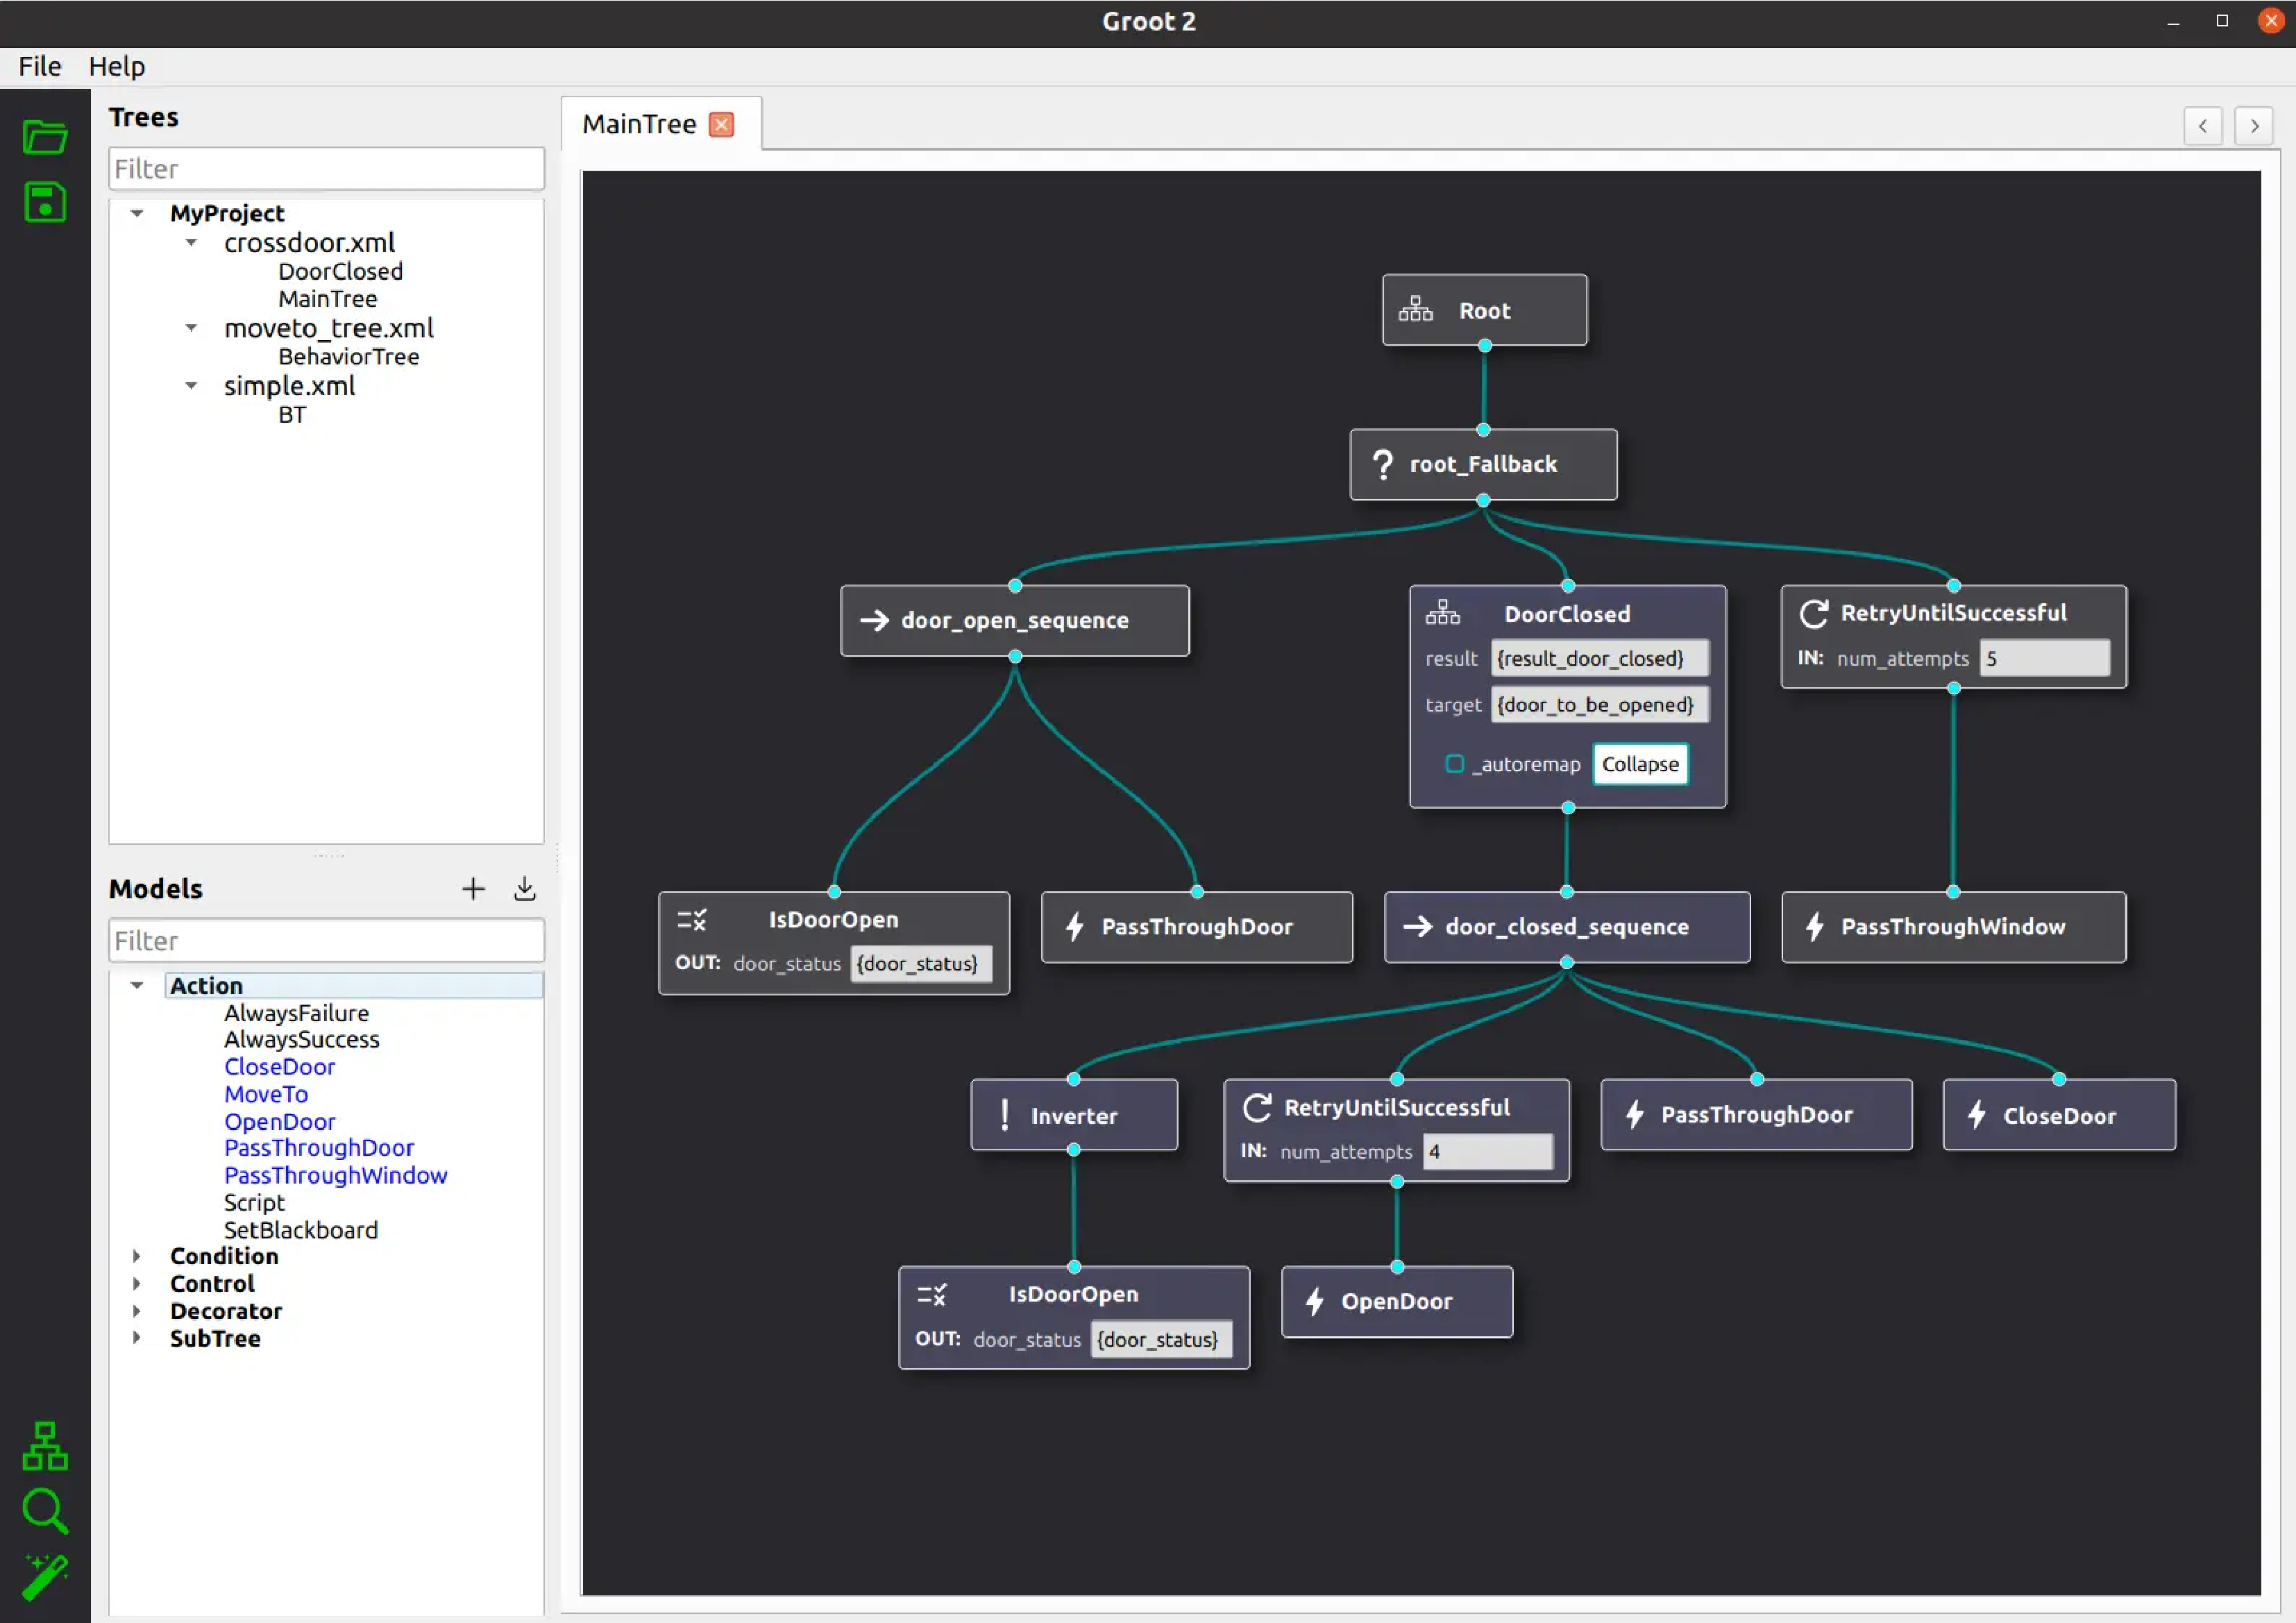
\includegraphics[width=0.75\linewidth]{images/Groot.pdf}
    \caption{Groot 2 interface. Taken from \cite{Groot}}
    \label{fig:groot}
\end{figure}

\subsection{Auxiliary Technologies}

In addition to the technologies used to build and debug the trees, other technologies are utilized in the context of the tree's operation, which will be elucidated as follows. These technologies were not chosen during the development of the new strategy, they were already employed by the ThunderVolt project and are part of its architecture as a whole.

Within this Subsection, these other technologies will be presented and their integration within the tree will be elucidated. This detailed explanation aims to facilitate a comprehensive understanding of how the tree is integrated with the rest of the system.

\subsubsection{Protobuf and UDP}

In the VSSS category, there are two tools that are important when testing and playing games, which are the FIRASim \cite{FIRASim}, a simulator used in the category, and the VSSReferee \cite{VSSReferee}, an automatic referee system which sends the game state and game control events to the teams playing a match. Both of these systems are crucial for the operation of the tree, as the simulator sends the states of the robots, which are used to decide when the roles of the robots should change, and the referee sends the events that define when the \texttt{Roles Swapper Initializer} tree (defined in Subsection \ref{subsec:roles_swapper_initializer_spec}) should be executed and how the initialization should be performed. 

In order to be able to communicate with those two systems, a protocol was defined by the category \cite{VSSProto} using Google's Protocol Buffers (\textit{Protobuf}) \cite{Protobuf}. The \textit{Protobuf} is a language-neutral and cross-platform framework to serialize data, so it can be stored or sent over a network. In the use case of the category, the serialized data is exchanged between the simulator, the referee and the teams playing the game using the User Datagram Protocol (UDP) \cite{rfc768}. The UDP is one of the core communication protocols of the internet, being a transaction oriented protocol, meaning that it does not require the network nodes to establish a connection to be able to communicate with each other. For the UDP-based communication, the team leveraged the capabilities of the \textit{Boost.Asio} library \cite{BoostAsio}, which is a cross-platform C++ library for network communication.

\subsubsection{ROS}

The Robot Operating System (\textit{ROS}) \cite{ROS} is a framework for developing robotics applications, it offers a diverse set of libraries and tools that help to build robotics projects. \textit{ROS} has a very large and global community, which helps to maintain all the libraries and to develop new algorithms, drivers and tools for the framework.

In the ThunderVolt project, \textit{ROS} is used to compose the structure of the whole software application, defining how the project will be executed, specifying the communication interface between all the different parts of the project that are performed in parallel, in addition to helping the system to be easily configurable and calibrated. In a less abstract way, for example, it is through ROS that the tree that is running in a separate process publishes the roles of the robots to the other processes that represent the robots, so they can execute the correct behavior.


\section{Implementation}
\label{sec:implementation}

This section will detail the implementation of the specification described in Section \ref{sec:specification}, highlighting the differences between what was previously specified and the final implementation.

Similar to Section \ref{sec:specification}, this section will first present the nodes that are common to some trees, then each subtree of the strategy tree will be briefly introduced and any implementation details will be elucidated. All images of nodes and trees shown in this section were created using the \textit{Groot 2} interface (see Subsubsection \ref{subsubsec:groot}).

\subsection{Common Nodes}
\label{subsec:common_nodes_impl}

The common nodes presented in this section are mostly very similar to the nodes presented in the Subsection \ref{subsec:common_nodes_spec}, changing just their representation. However, due to implementation details of the \textit{BehaviorTree.CPP} library, some of the nodes changed drastically and these changes will be clarified.

\subsubsection{Root Node}

The root node is represented as shown in Figure \ref{fig:root_node_impl}.

\begin{figure}[!h]
    \centering
    \includegraphics[width=0.15\linewidth]{chapters/development/images/RootNode.png}
    \caption{Root node in \textit{Groot}}
    \label{fig:root_node_impl}
\end{figure}

\subsubsection{Control Flow Nodes}

In contrast to the representation of control flow nodes discussed in Subsubsection \ref{subsubsec:control_nodes_spec}, the default behavior of a control flow node in the \textit{BehaviorTree.CPP} library is to be non-reactive. Therefore, as can be seen in Figure \ref{fig:control_nodes_impl}, nodes that deviate from this default behavior are specified as reactive nodes, rather than marking the non-reactive nodes differently. 

However, it is important to note that the \texttt{Sequence} node in this implementation differs slightly from the non-reactive sequence presented in Chapter \ref{ch:background}. When one of its children returns a failure, instead of ticking it again the next time the sequence is ticked, the whole sequence is restarted. The library also provides a sequence node with the same behavior of the sequence with memory as presented in Chapter \ref{ch:background}, but it was not used in the implementation of the tree. 

Additionally, another type of control flow node was used in the tree implementation, which is the decorator node, however, the reason why this node was used in the tree implementation will not be explained in this subsubsection, but in Subsubsection \ref{subsubsec:decator_nodes_impl}.

\begin{figure}[!h]
    \centering
    \begin{subfigure}[b]{.32\linewidth}
        \centering
        \includegraphics[width=0.52\linewidth]{chapters/development/images/FallbackNode.png}
        \caption{Non-reactive fallback}
    \end{subfigure}
    \hfill
    \begin{subfigure}[b]{.32\linewidth}
        \centering
        \includegraphics[width=0.57\linewidth]{chapters/development/images/SequenceNode.png}
        \caption{Non-reactive sequence}
    \end{subfigure}
    \hfill
    \begin{subfigure}[b]{.32\linewidth}
        \centering
        \includegraphics[width=0.8\linewidth]{chapters/development/images/ReactiveSequenceNode.png}
        \caption{Reactive sequence}
    \end{subfigure}
    \caption{Used control nodes representations in \textit{Groot}}
    \label{fig:control_nodes_impl}
\end{figure}

\subsubsection{Action Nodes}

The implementation of the common action nodes, in Figure \ref{fig:common_action_node_impl}, is very similar to the specification presented in Subsubsection \ref{subsubsec:common_action_nodes_spec}, the \texttt{Always Success} node is precisely the same and the node that sets a variable in the blackboard is a little bit different. 

In the tree specification, all blackboard variables were represented as strings or booleans, however, in the implementation, some of those variables were created as integer variables instead, therefore, two nodes that store variables in the blackboard were used, one that stores strings and another that stores integers. These two nodes have the same syntax, in the node, the \texttt{value} field receives the value to be stored in the blackboard and the \texttt{output\_key} receives the name of the variable in which the value will be stored. One thing important to note is that the node in Figure \ref{fig:set_blackboard_string_impl} is a built-in node of the library, while the node in Figure \ref{fig:set_blackboard_int_impl} is a custom node inspired by the node from the library.

\begin{figure}[!h]
    \centering
    \begin{subfigure}[b]{.32\linewidth}
        \centering
        \includegraphics[width=0.7\linewidth]{chapters/development/images/AlwaysSuccessNode.png}
        \caption{Always success}
    \end{subfigure}
    \hfill
    \begin{subfigure}[b]{.32\linewidth}
        \centering
        \includegraphics[width=0.85\linewidth]{chapters/development/images/SetBlackboardIntNode.png}
        \caption{Set Blackboard Int}
        \label{fig:set_blackboard_int_impl}
    \end{subfigure}
    \hfill
    \begin{subfigure}[b]{.32\linewidth}
        \centering
        \includegraphics[width=0.85\linewidth]{chapters/development/images/SetBlackboardStringNode.png}
        \caption{Set Blackboard String}
        \label{fig:set_blackboard_string_impl}
    \end{subfigure}
    \caption{Common used action nodes representation in \textit{Groot}}
    \label{fig:common_action_node_impl}
\end{figure}

\subsubsection{Condition Nodes}

In contrast to the tree specification, the common condition node specified in Subsubsection \ref{subsubsec:common_condition_nodes_spec} was not used in the tree implementation, decorator nodes were used instead, as it will be explained in the next subsubsection.

\subsubsection{Decorator Nodes}
\label{subsubsec:decator_nodes_impl}

The tree specification was created using condition nodes that verify whether the content of a variable in the blackboard is equal to a specified value, returning success or failure depending on the result of the assessment. However, the \textit{BehaviorTree.CPP} library does not provide a built-in condition node with the described behavior, instead, the library offers decorators that can be used for the same purpose.

Two decorators from the library were used to substitute the condition nodes, the \texttt{Blackboard Check Int}, in Figure \ref{fig:blackboard_check_int_impl}, and the \texttt{Blackboard Check String}, in Figure \ref{fig:blackboard_check_string_impl}. Both these nodes are very similar, they compare a value A with a value B, if both values are equal, this node will return the same status of its child otherwise it will return the value specified in the "return\_on\_mismatch" field. The difference between these two decorators is just the variable type that they handle, as the first handles integers and the second strings. One important thing to note is how these nodes actually access variables' values in the blackboard. This is accomplished by specifying the variable's name using the syntax \texttt{\{variable\_name\}}. By employing this syntax, the variable's value will be substituted during the comparison process, so it can be compared to the value in the other field.

\begin{figure}[!h]
    \centering
    \begin{subfigure}[b]{.49\linewidth}
        \centering
        \includegraphics[width=0.65\linewidth]{chapters/development/images/BlackboardCheckIntNode.png}
        \caption{Blackboard Check Int}
        \label{fig:blackboard_check_int_impl}
    \end{subfigure}
    \hfill
    \begin{subfigure}[b]{.49\linewidth}
        \centering
        \includegraphics[width=0.65\linewidth]{chapters/development/images/BlackboardCheckStringNode.png}
        \caption{Blackboard Check String}
        \label{fig:blackboard_check_string_impl}
    \end{subfigure}
    \caption{Blackboard Check decorator nodes representation in \textit{Groot}}
    \label{fig:common_decorator_nodes_impl}
\end{figure}

Regarding the use of these decorators, as it is not possible to simply replace a condition node with a decorator, it was necessary to make changes to the structure of the tree specification where the condition nodes which check the blackboard were used. To implement these modifications, an analysis of the structure which utilizes the \texttt{Blackboard Check} as a condition node was conducted, leading to the development of two alternative approaches using the \texttt{Blackboard Check} decorator implementation of the library.

Considering the tree specification, all the use cases of the \texttt{Blackboard Check} as a condition node can be abstracted as the two structures in Figure \ref{fig:blackboard_check_eq_condition_node}. The first structure, Figure \ref{fig:blackboard_check_eq_condition_node_fall}, represents the cases where the condition node is used as the first child of a non-reactive fallback, whereas the second structure, Figure \ref{fig:blackboard_check_eq_condition_node_seq}, represents the cases where the parent node of the condition node is a non-reactive sequence instead.

\begin{figure}[!h]
    \centering
    \begin{subfigure}[b]{.49\linewidth}
        \centering
        \scalebox{0.74} {
            \begin{forest}
                [\root, controlflow
                    [\fallback, controlflow
                        [{Blackboard Check \\ variable == value}, condition]
                        [{Conditional Action}, action]
                    ]
                ]
            \end{forest}
        }
        \caption{\texttt{Blackboard Check} as a condition node in a fallback}
        \label{fig:blackboard_check_eq_condition_node_fall}
    \end{subfigure}
    \hfill
    \begin{subfigure}[b]{.49\linewidth}
        \centering
        \scalebox{0.74} {
            \begin{forest}
                [\root, controlflow
                    [\sequence, controlflow
                        [{Blackboard Check \\ variable == value}, condition]
                        [{Conditional Action}, action]
                    ]
                ]
            \end{forest}
        }
        \caption{\texttt{Blackboard Check} as a condition node in a sequence}
        \label{fig:blackboard_check_eq_condition_node_seq}
    \end{subfigure}
    \caption{Tree structures abstraction when using the \texttt{Blackboard Check} as a condition node}
    \label{fig:blackboard_check_eq_condition_node}
\end{figure}

The first alternative to use the described decorator instead of the condition node can be seen in Figure \ref{fig:blackboard_check_eq_action_in_sequence}, in which the condition node is replaced by a decorator configured to return failure when there is a mismatch in the comparison and to return its child status, which will always be a success, when there is a match, mimicking the behavior of the condition node. This approach can be used as an alternative to both cases presented in Figure \ref{fig:blackboard_check_eq_condition_node}.

The second alternative, illustrated in Figure \ref{fig:blackboard_check_eq_action_as_child}, is a less verbose approach, using the decorator in a more standard manner, instead of using it to mimic the behavior of a condition node. As this solution requires fewer nodes than the first alternative, it presents itself as a better option. However, this approach cannot be used for both cases depicted in Figure \ref{fig:blackboard_check_eq_condition_node}, as its behavior only corresponds to the behavior of the structure in Figure \ref{fig:blackboard_check_eq_condition_node_seq}.

Therefore, the tree implementation, which will be presented in the next subsections, was structured in a way to adapt the tree specification using these alternatives. In the tree specification parts where the structure depicted in Figure \ref{fig:blackboard_check_eq_condition_node_fall} was utilized, the alternative approach illustrated in Figure \ref{fig:blackboard_check_eq_action_in_sequence} was employed to simulate a condition node. Conversely, in the parts where the structure depicted in Figure \ref{fig:blackboard_check_eq_condition_node_seq} is present, the alternative approach from Figure \ref{fig:blackboard_check_eq_action_as_child} was utilized.

\begin{figure}[!h]
    \centering
    \begin{subfigure}[b]{.49\linewidth}
        \centering
        \includegraphics[width=0.85\linewidth]{chapters/development/images/BlackboardCheck - Equivalence 1.png}
        \caption{\texttt{Blackboard Check} as a decorator with conditional action in sequence}
        \label{fig:blackboard_check_eq_action_in_sequence}
    \end{subfigure}
    \hfill
    \begin{subfigure}[b]{.49\linewidth}
        \centering
        \includegraphics[width=0.85\linewidth]{chapters/development/images/BlackboardCheck - Equivalence 2.png}
        \caption{\texttt{Blackboard Check} as a decorator with conditional action as child}
        \label{fig:blackboard_check_eq_action_as_child}
    \end{subfigure}
    \caption{Equivalent tree structures when using the \texttt{Blackboard Check} node}
    \label{fig:blackboard_check_equivalences}
\end{figure}

\subsubsection{Subtrees}

The representation of a subtree in the \textit{BehaviorTree.CPP} library, shown in Figure \ref{fig:subtrees_impl}, is very similar to the subtree specification described in the Subsubsection \ref{subsubsec:subtrees_spec}. The only notable difference between the two is that the library's implementation has an attribute called \texttt{\_\_shared\_blackboard}, which is used to specify whether the subtree will have its own blackboard or whether the tree which includes this subtree will share its blackboard with the subtree. In addition, the representation of a subtree node in \textit{Groot} also has a button that can be used to expand the subtree node and view the entire subtree.

\begin{figure}[!h]
    \centering
    \begin{subfigure}[b]{.49\linewidth}
        \centering
        \includegraphics[width=0.6\linewidth]{chapters/development/images/SubtreeNode - Not Shared BB.png}
        \caption{Subtree without shared blackboard}
    \end{subfigure}
    \hfill
    \begin{subfigure}[b]{.49\linewidth}
        \centering
        \includegraphics[width=0.6\linewidth]{chapters/development/images/SubtreeNode - Shared BB.png}
        \caption{Subtree with shared blackboard}
    \end{subfigure}
    \caption{Subtree node representation in \textit{Groot}}
    \label{fig:subtrees_impl}
\end{figure}

\subsection{Behaviors Controller Tree}

The \textit{Behaviors Controller} tree implementation, disregarding its subtrees, is basically the same as its specification, as it is possible to observe in Figure \ref{fig:behaviors_controller_bt_impl}, being the only notable difference the fact that it is now made explicit in the trees that they have a shared blackboard, by setting the \texttt{\_\_shared\_blackboard} attribute to true.

\begin{figure}[!h]
    \centering
    \includegraphics[width=0.7\linewidth]{chapters/development/images/BehaviorsController.png}
    \caption{Base structure implementation of the Coach’s Behavior Tree}
    \label{fig:behaviors_controller_bt_impl}
\end{figure}

\subsection{Roles Swapper Initializer}

In the implementation of the \texttt{Roles Swapper Initializer} tree, modifications were made to the tree specification, taking into account the information provided about the common nodes in Subsection \ref{subsubsec:common_action_nodes_spec}. The resulting implementation is depicted in Figure \ref{fig:roles_swapper_initializer_impl}. It is important to note that there is one implementation detail in this tree that deviates from its original specification, which is the data types of the variables stored in the blackboard.

\begin{figure}[!h]
    \centering
    \includegraphics[width=1.0\linewidth]{chapters/development/images/RolesSwapperInitializer.png}
    \caption{Roles Swapper Initializer subtree specification}
    \label{fig:roles_swapper_initializer_impl}
\end{figure}

In this tree and its subtrees, six blackboard variables are manipulated, which are the \texttt{game\_state}, the \texttt{game\_state\_team}, the \texttt{game\_state\_side}, the \texttt{use\_penalty\_mode}, the \texttt{use\_two\_strikers\_mode} and the \texttt{team\_state}.

In the tree specification, the \texttt{game\_state}, the \texttt{game\_state\_team}, and the \texttt{game\_state\_side} variables were all presented as strings for simplifications reasons, however, none of the real messages received from the \textit{VSSReferee} use strings to represent these data, just integers (see Tables \ref{tab:referee_events_ids}, \ref{tab:target_team_event_codification} and \ref{tab:field_side_event_codification}), therefore, the type of these variables in the blackboard was changed to integer.

The \texttt{use\_penalty\_mode} and the \texttt{use\_two\_strikers\_mode} variables were previously declared as booleans, nevertheless, to take advantage of the formerly developed \texttt{Set Blackboard Int} node, their data types were changed to integers as well, being \texttt{0} equivalent to \texttt{False} and \texttt{1} to \texttt{True}.

The last variable, the \texttt{team\_state}, did not have its data type changed, it remained a string as it is an internal variable of the tree, and keeping it as a string simplifies the tree and makes it more understandable.

\begin{table}[!htbp]
    \centering
    \begin{tabular}{c c}
        \toprule
        Event Name   & Value \\
        \midrule
        Free Kick    & 0     \\
        Penalty Kick & 1     \\
        Goal Kick    & 2     \\
        Free Ball    & 3     \\
        Kickoff      & 4     \\
        Stop         & 5     \\
        Game On      & 6     \\
        Halt         & 7     \\
        \bottomrule
    \end{tabular}
    \caption{Integer identifications of the events sent by the \textit{VSSReferee}, see \cite{VSSProto}}
    \label{tab:referee_events_ids}
\end{table}

\begin{table}[!htbp]
    \centering
    \begin{tabular}{c c}
        \toprule
        Target Team & Value \\
        \midrule
        Friends     & 0     \\
        Foes        & 1     \\
        \bottomrule
    \end{tabular}
    \caption{Codification, using the event and the team color, of the target team of the event received from the \textit{VSSReferee}}
    \label{tab:target_team_event_codification}
\end{table}

\begin{table}[!htbp]
    \centering
    \begin{tabular}{c c}
        \toprule
        Side of field & Value \\
        \midrule
        Friends' side & 0     \\
        Foes' side    & 1     \\
        \bottomrule
    \end{tabular}
    \caption{Codification, using the event and the team color, of the side of the field in which the event received from the \textit{VSSReferee} occurred}
    \label{tab:field_side_event_codification}
\end{table}

\subsection{Events Handler and its subtrees}

The \texttt{Events Handler} subtree has the same structure as its specification, being the only difference that it specifies the \texttt{\_\_shared\_blackboard} attributes of its subtrees. The implementation can be seen in Figure \ref{fig:events_handler_impl}.

\begin{figure}[!h]
    \centering
    \includegraphics[width=1.0\linewidth]{chapters/development/images/EventsHandler.png}
    \caption{Events Handler subtree implementation}
    \label{fig:events_handler_impl}
\end{figure}

Considering the changes presented in Subsection \ref{subsec:common_nodes_impl} and the changes to the data types of the variables on the blackboard, the implementations of all subtrees of the \texttt{Events Handler} subtree are analogous to their specifications. The implementations of the four subtrees are represented in Figures \ref{fig:penalty_kick_event_handler_impl}, \ref{fig:goal_kick_event_handler_impl}, \ref{fig:free_ball_event_handler_impl} and \ref{fig:kickoff_event_handler_impl}.

One simple implementation detail that deserves attention is the presence of parameters in the \texttt{Set Penalty Mode} node in the \texttt{Penalty Kick Event Handler}. These parameters were added to the node so it could be more generic, instead of having those values hardcoded into the node's code.

\begin{figure}[!h]
    \centering
    \includegraphics[width=0.7\linewidth]{chapters/development/images/PenaltyKickEventHandler.png}
    \caption{Penalty Kick Event Handler subtree implementation}
    \label{fig:penalty_kick_event_handler_impl}
\end{figure}

\begin{figure}[!h]
    \centering
    \includegraphics[width=0.9\linewidth]{chapters/development/images/GoalKickEventHandler.png}
    \caption{Goal Kick Event Handler subtree implementation}
    \label{fig:goal_kick_event_handler_impl}
\end{figure}

\begin{figure}[!h]
    \centering
    \includegraphics[width=0.9\linewidth]{chapters/development/images/FreeBallEventHandler.png}
    \caption{Free Ball Event Handler subtree implementation}
    \label{fig:free_ball_event_handler_impl}
\end{figure}

\begin{figure}[!h]
    \centering
    \includegraphics[width=0.65\linewidth]{chapters/development/images/KickoffEventHandler.png}
    \caption{Kickoff Event Handler subtree implementation}
    \label{fig:kickoff_event_handler_impl}
\end{figure}

\subsection{Roles Swapper}

Taking into account the insights discussed in Subsection \ref{subsec:common_nodes_impl}, the implementation of the \texttt{Roles Swapper} tree adheres closely to its specification, as depicted in Figure \ref{fig:roles_swapper_impl}.

\begin{figure}[!h]
    \centering
    \includegraphics[width=1.0\linewidth]{chapters/development/images/RolesSwapper.png}
    \caption{Roles Swapper subtree implementation}
    \label{fig:roles_swapper_impl}
\end{figure}

\subsection{Attack Swapper and Defense Swapper}

Finally, the \texttt{Attack Swapper} and \texttt{Defense Swapper} subtrees were also implemented taking into account the modifications discussed in Subsection \ref{subsec:common_nodes_impl}, the results are illustrated in Figures \ref{fig:attack_swapper_impl} and \ref{fig:defense_swapper_impl}, respectively.

Regarding the implementation of the nodes in both of these trees, it is noteworthy how the nodes that perform the roles changes and swaps were developed. To enhance the performance of the trees, these nodes were developed as asynchronous nodes, specifically using coroutines as their foundation. This design choice allows the role changes to be executed in parallel with the rest of the tree, without blocking its execution. The use of coroutines to develop the nodes was possible thanks to the \textit{BehaviorTree.CPP} library, which provides many ways of creating asynchronous nodes.

\begin{figure}[!h]
    \centering
    \includegraphics[width=1.0\linewidth]{chapters/development/images/AttackSwapper.png}
    \caption{Attack state internal swap subtree implementation}
    \label{fig:attack_swapper_impl}
\end{figure}

\begin{figure}[!h]
    \centering
    \includegraphics[width=1.0\linewidth]{chapters/development/images/DefenseSwapper.png}
    \caption{Defense state internal swap subtree implementation}
    \label{fig:defense_swapper_impl}
\end{figure}



\chapter{Results}
\label{ch:results}

In this chapter, the tests and results obtained from the implemented changes will be presented. A comprehensive comparison will be conducted between the new strategy and the old strategy, verifying whether all project requirements were fulfilled. To complete the comparison between the models, a detailed analysis of games played between the system using the old strategy and the system using the new one will be presented. Lastly, the chapter will include the results of applying the new strategy in a real robotics academic competition.

\section{Formal comparison between models}

To perform a formal comparison between the two models, it is necessary to take into account the design requirements presented in Chapter \ref{ch:requirements}.

First, considering the functional requirements of the project, the new strategy should be able to cover the same use cases as the previous model. When comparing the functions performed by the BT with those of the FSM, it is possible to observe that this requirement was fulfilled.

In the FSM, the events received from the referee were handled prior to the FSM start in order to decide which state would be the FSM entry state. There were five entry states, one for the attack state, one for the defense, one for when using two strikers instead of one, and two others for when a penalty occurred. This functionality was refactored when implementing the BT to integrate the definition of these configurations more seamlessly into the model, thus, blackboard variables were used that emulate the same behavior, as presented in Section \ref{sec:implementation}. In addition, the FSM also presented states to carry out role changes, which were incorporated into the tree in the \textit{RolesSwapper} subtree and on its subtrees. The role changes between the attack and the defense subgroups are carried out in the \textit{RolesSwapper} subtree itself, while the internal attack role changes are performed in the \textit{AttackSwapper} subtree and the defense role changes in the \textit{DefenseSwapper} subtree.

Regarding the non-functional requirements, the project successfully fulfilled all the specified requirements.

The system had its scalability improved both qualitatively and quantitatively. Previously, adding new functionality to the Coach or incorporating robots with different roles required defining specific states and managing all related transitions. However, with the new strategy, this process has become more flexible. The addition of new functionalities can now be achieved by utilizing blackboard variables to control the tree's flow. Similarly, introducing new robots with different roles only requires adding the specific nodes that handle the swaps of these roles to the \textit{AttackSwapper} or \textit{DefenseSwapper} subtrees and updating the nodes responsible for switching between attacking and defending roles.

In terms of system modularity, the model using a BT is significantly more modular than the model using the FSM. This fact becomes evident when examining the various subtrees that constitute the new strategy. In relation to human readability, it is possible to state that the graphical representation of the BT seems more complex than the representation of the FSM, but it is not the case.

The BT presents a more transparent structure of what is happening in the Coach, showing more clearly the entire process of changing roles, and the priority between the role changes. Additionally, the BT also incorporates the entire initialization part in the \textit{RolesSwapperInitializer} subtree, which was previously done more obscurely by defining the entry state of the FSM prior to the FSM execution.

\section{Tests between models}

To validate the effectiveness of the new strategy, a series of games were conducted between the system using the BT and the system using the FSM. Both teams were configured with identical settings, with the only distinction being the color used to identify them during the matches. A total of 250 games were played to evaluate the performance of the system. Each game consisted of two halves, each lasting five minutes, resulting in a cumulative total of 2500 game hours. All games were executed on a personal computer of the model Acer Aspire Nitro 5 with AMD Ryzen 7 4800H processor and 32GB of RAM memory. In this section, the setup to perform these tests will be explained, alongside the results of the games, and an analysis of the outcomes.

\subsection{Setup}

To better guarantee the equality of the two systems during the tests and enable the automation of the test execution, all test games between the two teams were carried out in a simulated way. Thus, the FIRASim simulator \cite{FIRASim} was used to simulate the environment, and the VSSReferee \cite{VSSReferee} was used to control the start of the game, the occurrence of fouls and define when the game ended.

In order to carry out the tests in an automated way, simplifying the validation process and the collection of metrics, it was necessary to use headless versions of both FIRASim and VSSReferee. However, the official version of VSSReferee does not yet support running headless, therefore a modified version of the system was used. The version used is currently a fork of the original repository, available on the ThundeRatz team's GitHub organization\footnote{https://github.com/ThundeRatz/VSSReferee}. Changes made to this repository were based on changes made to another fork\footnote{https://github.com/thiagohenrique1/VSSReferee}, by a member of the VSSS category community.

To facilitate the execution of the test system on any machine, \texttt{Docker}\footnote{https://www.docker.com/} and \texttt{Docker Compose}\footnote{https://docs.docker.com/compose/} were utilized to run FIRASim, VSSReferee, and the code from both teams. This approach allowed for a simple and efficient setup. Additionally, a bash script was created to automate the execution of the test system multiple times using \texttt{Docker Compose}.

\subsection{Evaluation}

The evaluation of the performance of the games between the two teams was made through the logs generated by VSSReferee. To read the log files, parse them and calculate performance metrics, a script was made using the Python language. The results of the games can be seen in Tables \ref{tab:wins}, \ref{tab:goals_number_metrics}, \ref{tab:goals_reasons}, and \ref{tab:fouls_count}.

In Table \ref{tab:wins}, it is possible to observe that most of the games between the two teams resulted in ties, however, the BT-based System had more wins than the FSM-based System.

\begin{table}[h]
    \centering
    \begin{tabular}{c c c}
        \toprule
        BT-based System Wins & Ties    & FSM-based System Wins \\
        \midrule
        34.80\%              & 42.40\% & 22.80\%               \\
        \bottomrule
    \end{tabular}
    \caption{BT-based system versus FSM-based system - Wins, losses and ties ratio}
    \label{tab:wins}
\end{table}

To better understand what happened during the games, metrics related to the number of goals scored by each team were collected and are presented in Table \ref{tab:goals_number_metrics}. It is noteworthy that the BT-based team scored more goals than the FSM-based team, a fact that can be demonstrated both by the total number of goals scored and the average number of goals per game achieved by each team. Additionally, the BT-based team achieved the highest number of goals in a single match. The last metric shown in the table is the average goal difference for each game, which reveals that, on average, the BT-based team had an advantage over the FSM-based team.

\begin{table}[h]
    \centering
    \begin{tabular}{l c c}
        \toprule
                                                       & BT-based System & FSM-based System \\
        \midrule
        Total goal                                     & 193             & 140              \\
        Maximum goals in a game                        & 5               & 3                \\
        Goals per game - average                       & 0.7720          & 0.5600           \\
        Goals per game - standard deviation            & 0.9550          & 0.7526           \\
        Goals difference per game - average            & 0.2120          & -0.2120          \\
        Goals difference per game - standard deviation & 1.1794          & 1.1794           \\
        \bottomrule
    \end{tabular}
    \caption{BT-based system versus FSM-based system - Metrics related to the number of goals}
    \label{tab:goals_number_metrics}
\end{table}

In addition, an analysis was also made of what caused the goals of each team. For this, the different types of events that the referee sends to the teams were taken into account. An event was considered to have caused a goal if the goal was scored within a margin of three seconds after the event occurred. The results of this analysis can be seen in Table \ref{tab:goals_reasons}. From these results, two differences stand out, the first being the difference in the number of penalty goals and the second the "other", which encompasses all other goals scored during the matches. This shows that the team with BT was able to take better advantage of penalty shots and plays in the middle of the game.

\begin{table}[h]
    \begin{minipage}{\columnwidth}
        \centering
        \begin{tabular}{l c c c c c}
            \toprule
                             & Free Ball & Penalty Kick & Goal Kick & Kickoff & Other \\
            \midrule
            BT-based System  & 20        & 28           & 1         & 0       & 143   \\
            FSM-based System & 21        & 8            & 0         & 0       & 111   \\
            \bottomrule
        \end{tabular}
        \begin{center}
            \footnotesize
            \emph{Note}: An event was considered as a cause of a goal if it occurred within three seconds after the event.
        \end{center}
    \end{minipage}
    \caption{BT-based system versus FSM-based system - Relationship of team goals with the events that caused them}
    \label{tab:goals_reasons}
\end{table}

Lastly, the total number of different events that occurred during a game was counted, these values are presented in Table \ref{tab:fouls_count}. The values shown for each team are very similar, however, some differences are noticeable. More \textit{Free Balls} occurred on the FSM-based side of the field than on the BT-based side, which may indicate that the ball stayed much longer in the FSM-based team's field, showing a more offensive position of the BT-based team. Besides that, more \textit{Penalty Kicks} events were received for the BT-based team, indicating that the FSM-based team committed more defensive fouls. Likewise, the BT-based team also received more \textit{Goal Kick} events, which may show that the FSM-based team also committed more attacking fouls. Finally, the FSM-based team received more \textit{Kickoff} events, which is expected given that the BT-based team scored more goals than the FSM-based team.

\begin{table}[h]
    \begin{minipage}{\columnwidth}
        \centering
        \begin{tabular}{l c c}
            \toprule
            Events        & BT-based System & FSM-based System \\
            \midrule
            Free Balls    & 2044            & 2152             \\
            Penalty Kicks & 335             & 318              \\
            Goal Kicks    & 137             & 115              \\
            Kickoffs      & 383             & 438              \\
            \bottomrule
        \end{tabular}
        \begin{center}
            \footnotesize
            \emph{Note}: In the case of Free Ball events, the name of the team refers \\
            to the side of the field where the foul occurred.
        \end{center}
    \end{minipage}
    \caption{BT-based system versus FSM-based system - Number of events received for each team}
    \label{tab:fouls_count}
\end{table}

\subsection{Discussion}

From the results presented, it is possible to affirm that the BT-based team, besides having improved the architecture of the team's coordination strategy by making the architecture more modular and scalable, also improved the team's performance during matches. The BT-based team managed to prevail in terms of number of goals, as well as being able to offer a more attacking posture and to make fewer fouls, in addition to being able to take better advantage of the opportunities to score goals with penalties.

This performance improvement can be demonstrated statistically as well. Considering that the goal difference of each game is calculated as the subtraction of the number of goals of the BT-based team by the number of goals of the FSM-based team, it is possible to make two hypotheses. The first, the null hypothesis ($H_0$), would be that the average goal difference of each game should be 0, in case both teams perform similarly, and the second hypothesis ($H_1$) would be that the average goal difference should be greater than 0, showing that the BT-based team performed better. This formulation can be seen in Equation \ref{eq:average_goals_diff_hypothesis}.

\begin{equation}
    \left\{
    \begin{aligned}
        H_0: \mu_0 = 0 \\
        H_1: \mu_0 > 0
    \end{aligned}
    \right.
    \label{eq:average_goals_diff_hypothesis}
\end{equation}

Using the previously presented values for the average goal difference and the standard deviation of the goal difference, it is possible to perform a one-sample t-test, obtaining a p-value of 0.00243. Considering a significance level of 5\%, it is possible to reject the null hypothesis and affirm that the BT-based team performed better than the FSM-based team.

This performance improvement may be explained by the better structuring of the strategy when using BTs, being able to define the priority between the role changes clearly, and having a more efficient way of verifying all the role swaps conditions. In addition, the reactivity of BTs may have also contributed to the team's performance, as the team was able to react more quickly to changes in the game state. Finally, it is important to note that, even though the goal of the new architecture was to cover the same use cases as the FSM-based architecture, the new strategy cannot be interpreted as a translation of the FSM strategy to BTs, but rather as a reinterpretation of the strategy, taking into account all the functionalities offered by BTs.

\section{Evaluation in robotics academic competition}

Given ThunderVolt's objective to compete at a high level with other teams, it is crucial that the implemented changes in the project have a positive impact on real competitions. Therefore, the changes presented in this work were tested in a Brazilian robotics academic competition, the IRONCup 2023 \cite{IRONCup2023}. The competition was held in February 2023 and in a virtual format, all games were played in the FIRASim simulator. The competition featured the participation of multiple teams including ThunderVolt, RobôCIn\footnote{https://robocin.com.br/}, Robotbulls\footnote{https://inatel.br/robotica/}, ITAndroids\footnote{https://www.itandroids.com.br/en/}, Red Dragons\footnote{https://www.linkedin.com/company/reddragons/}, Rinobot\footnote{https://www.linkedin.com/company/rinobot-team/}, and Neon\footnote{https://projectneon.dev/}.

The competition consisted of a round-robin tournament, that is, all teams faced each other once and accumulated points according to the games won. The tiebreaker between teams with the same number of points was the goal difference. The results of the games played by the ThunderVolt team are presented in Table \ref{tab:ironcup_games}, while the overall results of the competition are displayed in Table  \ref{tab:ironcup_results}. The ThunderVolt team won second place in the competition, proving the coordination structure's effectiveness.

\begin{table}[h]
    \centering
    \begin{tabular}{l c c c l}
        \toprule
        Blue team   &   &   &    & Yellow team \\
        \midrule
        ThunderVolt & 7 & x & 0  & Red Dragons \\
        Neon        & 0 & x & 14 & ThunderVolt \\
        ThunderVolt & 4 & x & 0  & ITAndroids  \\
        Rinobot     & 0 & x & 5  & ThunderVolt \\
        RobôCIn     & 3 & x & 0  & ThunderVolt \\
        Robotbulls  & 0 & x & 2  & ThunderVolt \\
        \bottomrule
    \end{tabular}
    \caption{Results of the games played by the ThunderVolt team \cite{ResultsIRONCup2023}}
    \label{tab:ironcup_games}
\end{table}

\begin{table}[h]
    \begin{minipage}{\columnwidth}
        \begin{center}
            \begin{tabular}{l c c c c c c c}
                \toprule
                Team        & Pts & GP & W & L & GS & GC & GD  \\
                \midrule
                RobôCIn     & 18  & 6  & 6 & 0 & 68 & 17 & 51  \\
                ThunderVolt & 15  & 6  & 5 & 1 & 32 & 3  & 29  \\
                Robotbulls  & 12  & 6  & 4 & 2 & 34 & 23 & 11  \\
                ITAndroids  & 9   & 6  & 3 & 3 & 36 & 17 & 19  \\
                Red Dragons & 6   & 6  & 2 & 4 & 36 & 36 & 0   \\
                Rinobot     & 3   & 6  & 1 & 5 & 14 & 54 & -40 \\
                Neon        & 0   & 6  & 0 & 6 & 7  & 46 & -39 \\
                \bottomrule
            \end{tabular}
        \end{center}
        \begin{center}
            \footnotesize
            \emph{Legend:} Pts: Points; GP: Games Played; W: Wins; L: Losses; GS: Goals Scored; \\GC: Goals Conceded; GD: Goal Difference.\\
            \emph{Points Count}: Each victory counts as three points and each tie counts as one point.
        \end{center}
    \end{minipage}
    \caption{Final results and ranking of the competition \cite{ResultsIRONCup2023}}
    \label{tab:ironcup_results}
\end{table}


\chapter{Final Considerations}
\label{ch:final_considerations}

\section{Conclusions}

This work demonstrated the feasibility of utilizing BTs to implement coordination strategies in multi-agent systems. Specifically, it showcased the successful implementation of a BT to define the behavior of the agent that is the leader of the MAS organization.

BTs provide a highly flexible, modular, and comprehensible control architecture that has significantly enhanced the system's scalability, maintainability, and adaptability to incorporate new functionalities, as adding new functionalities to the Coach's BT is much easier than adding new states in the previous FSM model. Therefore, in terms of architecture, BTs proved to be a great alternative to FSMs for defining complex behaviors of intelligent agents.

On the other hand, in terms of performance, the new strategy presented a subtle improvement to the system, observing a higher rate of victories over the team using the FSM. There are some factors that can justify this performance change.  Firstly, it should be noted that the BT implementation is not a direct translation of the previous FSM-based strategy, but rather a reinterpretation in light of the functionalities of BTs. In addition, something that can also have influenced the slightly better performance of the BT is the reactive nature of BTs and the greater ease in defining priorities between role changes in the new structure.

\section{Contributions}

The efforts put into this work have resulted in contributions in three main areas: the ThunderVolt project, the VSSS community, and the academic field.

Firstly, two major contributions were made to the ThunderVolt project, the first being the main focus of this work, which is the restructuring of the coordination strategy using BTs. The second contribution refers to the development of the test structure for the project, which greatly facilitates the validation of changes and enables a numerical analysis of the changes made.

Secondly, the contributions made to this work also impacted the VSSS community. In order to automate the tests using VSSReferee, the refereeing system had to be modified so that it could collect all game data when running the system without a graphical interface. These modifications are open-source and can be used by anyone in the VSSS community.

Lastly, this work extends the research on the use of BTs in multi-agent systems, especially in the context of dynamic allocation of tasks and task switching between the agents. This contribution was described in a paper that was submitted to the Intelligent Robotics and Multi-Agent Systems (IRMAS) track of the ACM Symposium on Applied Computing (SAC)\footnote{https://sac2024-irmas.isr.uc.pt/} and is currently under revision. This paper can be found in Appendix \ref{appendix:paper}.

\section{Continuity Prospects}

The ThunderVolt project is constantly changing to improve its performance and obtain better results in academic competitions. The changes made in this work ensure a better project structure and improved maintainability. The improvement made the project more flexible to changes so that the system coordination strategy can be improved even further later, in order to have a greater impact on the performance of the team.

Additionally, the introduction of an automated testing system and the development of a script for collecting metrics have added significant value to the project. These tools enable the team to validate and evaluate the impact of the changes made. These testing and metrics collection capabilities open up the possibility for investing in machine learning techniques that can be combined with the developed BT to further improve the system's performance.


% ========== Glossary and References ==========

\nocite{*}

\printbibliography[heading=bibintoc, title=References]

% ========== Appendix ==========

\appendix

\chapter{Paper SAC'24}
\label{appendix:paper}

This appendix presents the paper submitted to the Intelligent Robotics and Multi-Agent Systems (IRMAS) track of the ACM Symposium on Applied Computing (SAC), currently being under review.

\includepdf[pages=-,pagecommand={}]{appendices/Paper_ACM_Coordinating_a_Robotics_Multi_Agent_System_Using_Behavior_Trees.pdf}

\chapter{ThunderVolt TDP}
\label{appendix:tdp}

This appendix contains the Team Description Paper (TDP) of the ThunderVolt team, presented as a requirement for participation in the Latin American Robotics Competition (LARC) 2021 competition. This paper is referenced in this work by \cite{TDPThunderVolt}.

\includepdf[pages=-,pagecommand={}]{appendices/ThunderVolt_TDP_LARC_2021.pdf}


\end{document}
